% SPDX-License-Identifier: GPL-2.0-or-later
% Blendity: the architecture book (task 0386). Build: python tools/make_books.py --pdf (lualatex + biber).
% The language a reader and a search index read. Structure tags (tagging=on) are off: LaTeX's
% tagging project does not yet support the packages used (tcolorbox, titlesec), so the figures carry captions and alt text instead.
\DocumentMetadata{lang=en-GB}
\documentclass[11pt, twoside, openany]{book}
\usepackage{blendity-common}
\graphicspath{{figures/}{../images/}}

\title{Blendity: Architecture and Engineering}
\author{Emiliano Manalo, with Anthropic's Claude}
\date{Version 0.13.0, November 2026}

\hypersetup{pdftitle={Blendity: Architecture and Engineering}, pdfauthor={Emiliano Manalo}, pdfsubject={How Blendity is built, tested and released}}

\begin{document}
\frontmatter
\begin{titlepage}
  \centering
  \vspace*{30mm}
  {\sffamily\bfseries\Huge Blendity\par}
  \vspace{6mm}
  {\sffamily\LARGE Architecture and Engineering\par}
  \vspace{4mm}
  {\sffamily\large How the editor is built, how it is developed with an AI under human review, and how it is tested and released\par}
  \vspace{18mm}
  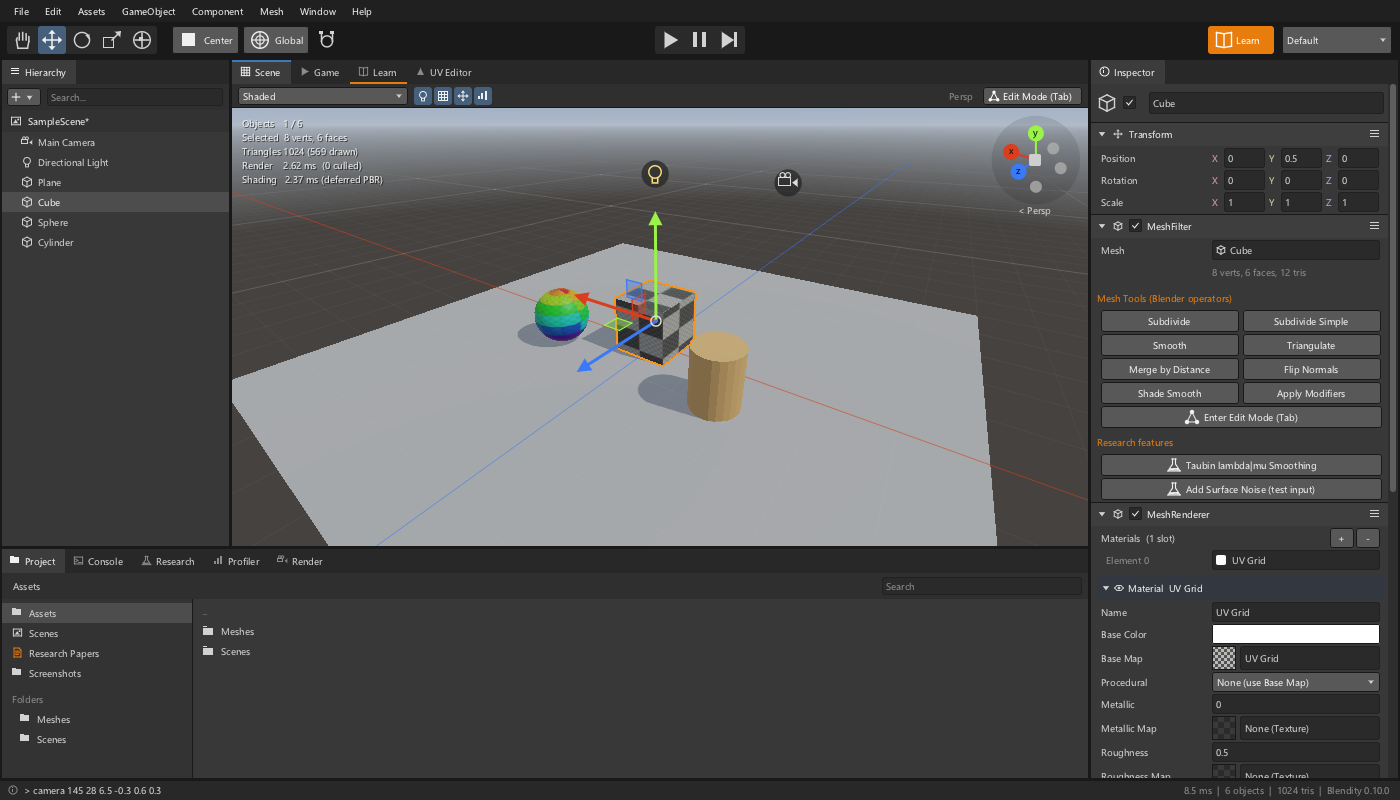
\includegraphics[width=0.86\textwidth, alt={The Blendity editor: the Hierarchy on the left, the Scene view in the middle with a path-traced scene, the Inspector on the right, the Project and Console windows along the bottom.}]{editor.png}\par
  \vspace{14mm}
  {\sffamily Emiliano Manalo, with Anthropic's Claude\par}
  {\sffamily Version 0.13.0 \quad November 2026\par}
  \vfill
  {\sffamily\footnotesize Source: GPL-2.0-or-later. Binaries: GPL-3.0-or-later. \url{https://github.com/EmilianoManaloIV/blendity}\par}
\end{titlepage}

\chapter*{About this book}
\addcontentsline{toc}{chapter}{About this book}
This book is for someone who wants to understand how Blendity works well enough to change it: a contributor, a reviewer,
a student of how an editor of this size is put together, or a maintainer years from now. It describes the program as it
stands at version 0.13.0 and the way it was made, with every borrowed idea, library and paper credited in the References
chapter and three indexes that tie the code, the user interface and the documents to those references.

It is written once, as the user asked, rather than re-edited every round; the living documents it condenses
(\code{docs/ARCHITECTURE.md}, \code{docs/decisions/}, \code{docs/tasks/}, \code{CHANGELOG.md}) stay the record of what
changed since. Where this book and those files disagree, the files are newer.

The companion volume, \emph{Blendity: The User Guide}, is for the artist: how to navigate the editor and how to feel at
home in it coming from Unity, Blender, Maya, 3ds Max, SketchUp, Unreal or Adobe's tools.

\tableofcontents
\listoffigures

\mainmatter
\chapter{Purpose and scope}
\label{ch:purpose}

\section{What Blendity is}
Blendity is a 3D editor written in C++17. Its windows, navigation, shortcuts, gizmos, Inspector and Play mode follow
the Unity editor \cite{UnityManual2026}; underneath, its meshes, Edit Mode tools, UV unwrapping, Principled materials,
render engines (an EEVEE-like rasterizer and a Cycles-like path tracer on the CPU and any Vulkan GPU), skins and IK
follow Blender's design and source code \cite{Blender2026}. It is not a fork: each subsystem is re-implemented, following
Blender's design, so the editor builds and runs with nothing but a compiler, and the matching Blender source file is
listed for every module. When Blender's prebuilt libraries are present it links the same ones Blender uses, each behind
a switch with Blendity's own code as the fallback (\adr{0001}).

It is one process with no plugins and no scripting runtime. Three executables share one static library built from
\code{src/}: \code{Blendity} (the editor), \code{blendity\_tests} and \code{blendity\_stress}. Everything a tool does is
reachable from the Console's command line, which is how the tests, the headless mode and the HCI harnesses drive it.

\section{Who it is for}
The requirements (\code{docs/requirements.md}) name the audience by what they must be able to do: a Unity-style editor
(R-01) with Blender-equivalent modeling (R-02) and SketchUp / UModeler / Plasticity-style direct modeling (R-03), UVs,
materials and textures (R-04), rendering with both engines (R-05), file formats matching Blender 5.2 (R-06), every tool
reachable from menus, panels, rebindable shortcuts and the console (R-07), adjustable operations (R-08), a Learn tab
(R-09), camera filters (R-10), Unity-like global illumination (R-11, R-12), physics for animation as in Cascadeur
(R-13), fingers and a pen on a 2-in-1 (R-14), and drawing in perspective with the model built from construction lines
(R-15). The HCI reports in \code{docs/hci/} measure the editor with artists from Unity, Unreal and Adobe's tools in
mind, on keyboard, pen and tablet; the later rounds added the VRChat avatar and world pipelines, with the editor
reading and writing Unity's own project files.

\section{What this book covers}
Chapters~\ref{ch:context} to \ref{ch:bridges} describe the system: its context, the layers and the two flows that
organise everything (one frame, one edit), the scene and mesh model, rendering, the editor toolkit, and the bridges to
other programs. Chapter~\ref{ch:research} lists the research features and where each paper landed. Chapters~\ref{ch:sdlc}
to \ref{ch:performance} describe how the program is made: the agentic software development lifecycle with its
artifacts and gates, the build, test and release machinery, and the performance work. Chapter~\ref{ch:scope} says what
is not recreated. Chapter~\ref{ch:licensing} states the licence and the credits. The References chapter and the two
indexes close the book.

\section{Conventions}
\code{Monospace} is a file, a function, a flag or a console command; paths are relative to the \code{blendity/} folder
unless they start with \code{blender/}, which is Blender's source tree beside the project. \adr{NNNN} is a decision
record in \code{docs/decisions/}, \task{NNNN} a specification in \code{docs/tasks/}, and \rnd{NNN} an entry of
\code{CHANGELOG.md} (one entry per round of requests). Numbers quoted here were measured on the machines the CHANGELOG
names; where a figure is an estimate, the text says so.

\section{The numbers at 0.13.0}
\begin{center}
\begin{tabular}{lr}
\toprule
Source files under \code{src/} (C++, headers, Objective-C++, CUDA) & 380 \\
Lines in \code{src/} & about 297,000 \\
Lines of unit tests (\code{tests/}) & about 73,600 \\
Unit checks / tests, the build with Blender's libraries & 15,902 / 1,543 \\
Unit checks, the dependency-free build (Windows and Linux) & 15,253 / 15,259 \\
Test groups (\code{--group}) & 16 \\
Decision records & 104 \\
Task specifications & 379 \\
Rounds in the CHANGELOG & 409 \\
Learn lessons & 45 \\
Windows (module registry) & 26 \\
Keymap presets / editor feels & 7 / 4 \\
Commits on \code{main} since 2026-10-06 & 436 \\
\bottomrule
\end{tabular}
\end{center}

\chapter{Context}
\label{ch:context}

\begin{figure}[H]
  \centering
  \resizebox{\textwidth}{!}{% The system context: Blendity, the people and programs around it.
\begin{tikzpicture}[node distance=9mm and 12mm]
  \node[box, fill=blAmber!15, draw=blAmber, minimum width=52mm, minimum height=22mm, align=center] (bl)
    {\textbf{Blendity}\\[1pt] \footnotesize one process, no plugins, no scripting runtime\\ \footnotesize the editor, \code{blendity\_tests}, \code{blendity\_stress}};
  \node[person, above=of bl] (artist) {The artist\\ \footnotesize keyboard, mouse, pen, fingers, a VR headset};
  \node[ext, left=18mm of bl, align=center] (os) {Windows / Linux / macOS\\ \footnotesize one window, input, files,\\ \footnotesize the trash, dialogs};
  \node[ext, below left=12mm and -6mm of bl, align=center] (gpu) {Any Vulkan GPU\\ \footnotesize (OptiX on NVIDIA)};
  \node[ext, below=of bl, align=center] (libs) {Blender's prebuilt libraries\\ \footnotesize optional, behind \code{BL\_WITH\_*}};
  \node[ext, below right=12mm and -6mm of bl, align=center] (dl) {Optional downloads\\ \footnotesize the libraries, AI inbetweening, MoonRay};
  \node[ext, right=18mm of bl, align=center] (engines) {Blender, Unity, Godot, Unreal\\ \footnotesize Live Link bridges (TCP, loopback)\\ \footnotesize files: OBJ, FBX, glTF, STL, PLY, USD,\\ \footnotesize .unitypackage, .tscn, .blend};
  \node[ext, above right=8mm and 2mm of bl, align=center] (gh) {GitHub\\ \footnotesize releases, the daily update check};
  \node[ext, above left=8mm and 2mm of bl, align=center] (proj) {The project folder\\ \footnotesize \code{Assets/}, scenes, materials, renders};
  \draw[flow, <->] (artist) -- (bl);
  \draw[flow, <->] (os) -- (bl);
  \draw[flow] (bl) -- (gpu);
  \draw[dflow] (libs) -- (bl);
  \draw[dflow] (dl) -- (bl);
  \draw[flow, <->] (bl) -- (engines);
  \draw[dflow] (gh) -- (bl);
  \draw[flow, <->] (proj) -- (bl);
\end{tikzpicture}
}
  \caption{The system context. Solid arrows are data both ways or out; dashed arrows are optional inputs Blendity runs without.}
  \label{fig:context}
\end{figure}

\section{The people}
One artist at a time, at a desk or on a 13-inch 2-in-1, with a keyboard and a mouse, a pen, fingers on the screen, a
pen display with a dial and express keys, or an OpenXR headset. The HCI work (\adr{0085}) names the artists it designs
for: people arriving from Unity, Unreal, Blender and Adobe's tools, keyboard-first and pen-first. The one developer is
the user, working with an AI (chapter~\ref{ch:sdlc}).

\section{The operating system}
\code{src/platform} is one window and its input on Win32, X11 (with XInput~2 for pens and touch) and Cocoa, plus the
clipboard, native file dialogs, the trash and DPI, mirroring Blender's GHOST layer \cite{Blender2026}. Everything above
it is portable C++17 built by \code{build.bat} on Windows (MSVC, found automatically) and \code{build.sh} on Linux and
macOS, with CMake optional (C-01). Pixels are \code{0xAARRGGBB} so all three can blit without conversion; the editor
redraws only on input, animation or timers and otherwise sleeps in the OS event wait.

\section{The GPU}
Any Vulkan 1.2 GPU: the loader is opened at run time (\code{VK\_NO\_PROTOTYPES}), so a machine without one runs on the
CPU. The GPU does three things, each with a CPU equivalent: the views are drawn by \code{gpu::Raster} with the CPU's
formulas in GLSL (\adr{0061}); the path tracer runs its kernel as a Vulkan compute shader (hardware ray queries where
they exist) or, on NVIDIA cards, through OptiX (\adr{0037}, \adr{0054}); and lighting bakes gather on it. CPU and GPUs
render together, claiming samples from one counter.

\section{Blender's libraries, optional}
When \code{blender/lib/<platform>} exists beside the project, the build links Blender's own prebuilt libraries
(Embree, OpenImageDenoise, oneTBB, Eigen, OpenSubdiv, OpenEXR, OpenColorIO, Manifold, meshoptimizer, Open PGL, Jolt,
Vulkan + shaderc, FFmpeg and others), each behind \code{BL\_WITH\_<NAME>} with a fallback (\adr{0001}, C-02).
\code{BLENDITY\_NO\_LIBS=1} forces the dependency-free build, which CI tests on every system; the installers ship both
programs and Blendity hands over to Blendity-full when the libraries load (\adr{0033}). The Console's \code{libs} prints
what a build has.

\section{Files and other programs}
A project is a folder with \code{Assets/} inside, as Unity's (\code{BlendityProject} in the home folder unless another is
opened). Scenes are text (\code{.scene}, Zstandard-compressed when the library is there), materials \code{.mat},
procedural textures \code{.ptex}, clips \code{.anim}, sequences \code{.seq}, layouts \code{.blendity-ui}. Models move
through OBJ, FBX, glTF, STL, PLY and USD, verified both ways against Blender 5.2 (R-06), and through Unity's
\code{.unitypackage}, \code{.prefab}, \code{.unity}, \code{.mat} and \code{.anim}, Godot's \code{.tscn} and Blender's
\code{.blend} (through the installed Blender). Live Link streams the scene to Blender, Unity, Godot and Unreal on the
same computer as it changes (chapter~\ref{ch:bridges}).

\section{The network}
Two uses, both optional and both the user's choice: a once-a-day check of GitHub's releases for a newer build
(\code{src/core/releases.cpp}; Preferences $>$ Updates), and Live Link's TCP server on 127.0.0.1 (no other computer can
connect; it is one way out). There is no telemetry and no cloud; the only learned model in the product is the optional,
local AI inbetweening download (\adr{0046}).

\section{The programs it follows}
The context has a second ring: the programs whose ideas the editor reproduces, each credited in chapter~\ref{ch:licensing}
and \code{CREDITS.md}. Unity for the editor's shape, Blender for the data and the tools, SketchUp, UModeler and
Plasticity for direct modeling, ZBrush and Sculptris for sculpting, Substance Painter for texturing, SketchBook, Photoshop
and Krita for drawing, Mixamo and the CATS plugin for rigging and avatars, Cascadeur for physics in animation, Premiere
for the sequencer, Lightroom for the Editing tab, Unity's Mecanim for retargeting. Where Blendity differs from them, the
user guide says so at the moment it matters.

\chapter{Architecture}
\label{ch:architecture}

\section{Layers}
\begin{figure}[H]
  \centering
  \resizebox{\textwidth}{!}{% The module layers of src/: each depends only on the ones below it.
\begin{tikzpicture}[node distance=3mm]
  \node[layer, minimum width=150mm, fill=blAmber!15, draw=blAmber, text width=146mm] (editor)
    {\textbf{editor} \quad the IMGUI toolkit (\code{ui::Context}), docking, the 26 windows, tools, keymaps, undo, Live Link, the Learn tab, the console};
  \node[layer, minimum width=150mm, below=of editor, text width=146mm] (render)
    {\textbf{render} \quad canvas and fonts, the rasterizer, the path tracer, GPU devices (Vulkan, OptiX), colour management, lightmaps, probes, voxel GI, camera filters};
  \node[layer, minimum width=72mm, below left=3mm and -72mm of render, text width=68mm] (texture) {\textbf{texture} \quad procedural stacks, surfaces, smart materials};
  \node[layer, minimum width=72mm, right=6mm of texture, text width=68mm] (research) {\textbf{research} \quad paper-derived features behind a registry};
  \node[layer, minimum width=150mm, below=14mm of render, fill=blMint!12, text width=146mm] (scene)
    {\textbf{scene} \quad Mesh (Blender's layout) and \code{meshops}, UVs, materials, modifiers, GameObject / components, the Reflector, IO, skins, IK, clips, physics};
  \node[layer, minimum width=72mm, below left=3mm and -72mm of scene, text width=68mm] (image) {\textbf{image} \quad codecs, mipmapped textures};
  \node[layer, minimum width=72mm, right=6mm of image, text width=68mm] (platform) {\textbf{platform} \quad one window + input: Win32 / X11 / Cocoa};
  \node[layer, minimum width=150mm, below=14mm of scene, fill=blBlue!10, text width=146mm] (core)
    {\textbf{core} \quad math (Unity's conventions), hashes, logging, filesystem, jobs (TBB or own pool), CPU features, the frame pacer, the net server};
  \node[layer, minimum width=72mm, below left=3mm and -72mm of core, text width=68mm, fill=blCode] (deps) {\textbf{deps} \quad which libraries were built in (\code{libs})};
  \node[layer, minimum width=72mm, right=6mm of deps, text width=68mm, fill=blCode] (app) {\textbf{app} \quad \code{main()}, the headless entry points};
  \draw[flow] (editor) -- (render);
  \draw[flow] (render) -- (texture);
  \draw[flow] (render) -- (research);
  \draw[flow] (texture) -- (scene);
  \draw[flow] (research) -- (scene);
  \draw[flow] (scene) -- (image);
  \draw[flow] (scene) -- (platform);
  \draw[flow] (image) -- (core);
  \draw[flow] (platform) -- (core);
  \node[note, below=2mm of deps.south west, anchor=north west, text width=146mm] {\code{scene} never includes \code{editor} or \code{render}: mesh operators are pure functions on a \code{Mesh} plus selection vectors, which is what lets the tests and the stress suite call them directly. \code{deps} and \code{app} are the two small modules that see everything.};
\end{tikzpicture}
}
  \caption{The layers of \code{src/}. Each depends only on what is below it; the side modules are small and sit beside the stack.}
  \label{fig:layers}
\end{figure}

\begin{center}
\begin{tabularx}{\textwidth}{lXl}
\toprule
Layer & Owns & Depends on \\
\midrule
\code{core} & math (Unity's left-handed, Y-up conventions), hashes (FNV-1a and the per-frame mixer), logging, the filesystem, jobs (TBB or its own pool), CPU features, the frame pacer, the TCP server & -- \\
\code{platform} & one window, input events, clipboard, file dialogs, the trash (Win32 / X11 / Cocoa) & core \\
\code{image} & PNG, JPEG, TGA, BMP, HDR decoding (EXR with OpenEXR), JPEG / HDR / PNG encoding, mipmapped textures & core \\
\code{scene} & \code{Mesh} (Blender's corner-based layout) and the \code{meshops} operators, UVs, materials, modifiers, \code{GameObject} / components, scene and model IO, skins, IK, animation clips, sequences, physics, sketch data & core, image \\
\code{texture} & procedural texture stacks, surfaces (the layer stack on an object), smart materials & scene \\
\code{render} & 2D canvas and fonts, the rasterizer, the path tracer, GPU devices, colour management, lightmaps, probes, voxel GI, mesh maps, camera filters, video encoding & core, image, scene \\
\code{editor} & the IMGUI toolkit (\code{ui::Context}), docking, the windows, tools (draw, knife, push/pull, modal transforms, sculpt, paint, sketch), keymaps, undo, Live Link, the Learn tab, the console & everything above \\
\code{research} & paper-derived features behind a registry (cited in Learn $>$ References) & scene \\
\code{deps}, \code{app} & which libraries were built in (the \code{libs} command); \code{main()} and the headless entry points & all \\
\bottomrule
\end{tabularx}
\end{center}

\code{scene} never includes \code{editor} or \code{render}. Mesh operators (\code{meshops::*}, in
\code{src/scene/mesh\_tools*.cpp}) are pure functions on a \code{Mesh} plus selection vectors, which is what lets the
tests and the stress suite call them directly, and what keeps the editor a thin layer of intent over the data.

\section{One frame}
\code{platform} events $\to$ \code{Editor::frame} $\to$ the windows draw and handle input in docking order (the Scene
view runs the active tool: \code{draw\_update}, \code{pushpull\_update}, \code{modal\_update}, the gizmo) $\to$
\code{handle\_shortcuts} (the keymap; tools consume the keys they own first) $\to$ the frame is rasterized into the
editor's framebuffer $\to$ \code{platform} presents it, only the 16-row bands whose pixels changed. Headless runs
(\code{init\_headless} + \code{step\_frame\_headless}) execute the same frame without a window; the tests drive the UI this
way with synthetic mouse and key events, and \code{Blendity --headless-screenshot} runs console commands and writes a
picture. A \code{FramePacer} (\code{src/core/pacer.h}) starts frames at most \code{1 / max\_fps} apart without oversleeping
\cite{Gregory2018vol1}.

\section{One edit}
\begin{figure}[H]
  \centering
  \resizebox{\textwidth}{!}{% One edit: from a tool to an undo step, through copy-on-write meshes and the Reflector.
\begin{tikzpicture}[node distance=6mm and 8mm]
  \node[box] (tool) {A tool, a menu,\\ the console's \code{editop}};
  \node[box, right=of tool] (edit) {\code{Editor::edit\_tool(op)}};
  \node[box, right=of edit] (mut) {\code{mesh\_make\_mutable}\\ \footnotesize clones a shared mesh};
  \node[box, right=of mut] (ops) {\code{meshops::*}\\ \footnotesize a pure function on\\ \footnotesize Mesh + selection};
  \node[box, below=of ops] (touch) {\code{Mesh::touch()}\\ \footnotesize version++};
  \node[box, below=of mut] (last) {\code{LastOp}\\ \footnotesize \code{before}, the numbers,\\ \footnotesize the result's version};
  \node[box, below=of edit] (mark) {\code{mark\_changed}\\ \footnotesize one undo step: a scene clone\\ \footnotesize sharing unchanged meshes};
  \node[box, below=of tool] (f9) {F9 / the drag helper\\ \footnotesize \code{run\_last\_op}: re-runs from\\ \footnotesize a copy of \code{before}};
  \node[box, below=12mm of mark, fill=blCode] (caches) {Version-keyed caches\\ \footnotesize render mesh, edge table, overlap check,\\ \footnotesize the views' pictures (\code{scene\_render\_hash})};
  \node[box, below=12mm of touch, fill=blCode] (refl) {\code{Reflector}\\ \footnotesize one field description drives the\\ \footnotesize Inspector, files, undo and hashing};
  \draw[flow] (tool) -- (edit);
  \draw[flow] (edit) -- (mut);
  \draw[flow] (mut) -- (ops);
  \draw[flow] (ops) -- (touch);
  \draw[flow] (ops.south west) -- (last.north east);
  \draw[flow] (touch) -- (mark);
  \draw[flow] (mark) -- (f9);
  \draw[flow, <->] (f9) -- (last);
  \draw[dflow] (touch) -- (caches);
  \draw[dflow] (mark) -- (refl);
\end{tikzpicture}
}
  \caption{One edit, from a tool to an undo step. Solid arrows are the call path; dashed arrows are what the edit's version bump reaches.}
  \label{fig:edit}
\end{figure}

A tool or menu calls \code{Editor::edit\_tool(op)} (or the console's \code{editop}). Operators that take numbers become a
\code{LastOp}: \code{run\_last\_op} copies \code{LastOp::before}, applies the \code{meshops} function with the current
values, records the result's pointer and version, and the F9 panel or the drag helper re-runs it when a value changes.
\code{mark\_changed} turns the edit into one undo step: a scene clone sharing the unchanged meshes (\adr{0003}).

\section{Invariants}
\begin{rulebox}{What every change must keep}
\begin{itemize}
  \item \textbf{Copy-on-write meshes} (\adr{0003}): \code{mesh\_make\_mutable} before writing; re-read \code{MeshPtr}
    after an edit; every change \code{touch()}es the mesh so version-keyed caches refresh. A redoable operator's
    \code{LastOp::before} is the undo step's pointer, never written: \code{run\_last\_op} makes the operator's one copy
    (\adr{0053}).
  \item \textbf{Edit Mode selections} are vectors indexed like the mesh (\code{vert\_sel\_}, \code{face\_sel\_}) plus a set
    of edge keys (\code{edge\_sel\_}); any operator that renumbers faces or vertices rebuilds them.
  \item \textbf{Adjustable operations} re-run from \code{before}; anything that changes the result after it was recorded
    must update \code{LastOp::result\_version} (\adr{0005}), or F9 treats the operation as gone.
  \item \textbf{Geometry robustness} (Q-01): operators leave a structurally valid mesh or refuse with a message; closed
    meshes stay closed; no new faces lying on top of each other without an explanation (Q-02, counted by the stress suite).
  \item \textbf{Isolation of user files} (C-04): tests and stress run in a scratch project and trash
    (\code{BLENDITY\_PROJECT}, \code{BLENDITY\_TRASH}); nothing they do touches \code{Assets/}.
  \item \textbf{No main-thread stalls}: heavy work (bakes, remeshes, skin binds, Live Link's payloads, texture
    evaluation) runs on workers with a cancel flag and shows in the job tray; the views keep their last picture
    meanwhile (\adr{0039}, \adr{0095}).
  \item \textbf{Every tool is reachable from the console} (\code{editop}, \code{edittool}, \code{drawpoint}, \ldots),
    so tests and scripts can drive it, and \code{tools/test\_coverage\_map.py --check} finds no command, keymap action or
    window without a test (\adr{0056}).
\end{itemize}
\end{rulebox}

\section{Module map}
\code{docs/ARCHITECTURE.md} keeps the full map, one row per subsystem with the Blender source file it mirrors and the
Unity equivalent; this is the shape of it.

{\small
\begin{longtable}{>{\raggedright\arraybackslash}p{0.27\textwidth}>{\raggedright\arraybackslash}p{0.42\textwidth}>{\raggedright\arraybackslash}p{0.24\textwidth}}
\toprule Blendity & What it does & Blender source it mirrors \\ \midrule \endfirsthead
\toprule Blendity & What it does & Blender source it mirrors \\ \midrule \endhead
\bottomrule \endfoot
\code{core/math.h} & vectors, quaternions, column-major matrices; Unity's left-handed Y-up, ZXY Euler & \code{blenlib/BLI\_math\_matrix.hh} \\
\code{core/jobs.*} & \code{parallel\_for}: oneTBB when available, else its own pool & \code{blenlib/BLI\_task.hh} \\
\code{render/canvas.*} & UI drawing, anti-aliased TrueType text from OS fonts & \code{blenfont/intern/blf\_glyph.cc} \\
\code{render/raster.*} & tile-binned multithreaded rasterizer, z-buffer, id buffer, outlines & \code{draw/intern/draw\_manager.cc}, \code{gpu/intern/gpu\_select.cc} \\
\code{scene/mesh.*} & \code{positions} + \code{face\_offsets} + \code{corner\_verts} (n-gons), render cache & \code{makesdna/DNA\_mesh\_types.h}, \code{blenkernel/BKE\_mesh.hh} \\
\code{mesh\_make\_mutable} & copy-on-write sharing & \code{blenlib/BLI\_implicit\_sharing.hh} \\
\code{meshops::*} & extrude, inset, bevel, bridge, loop cut, knife, dissolve, fill, spin, slice, push/pull, \ldots & \code{bmesh/operators}, \code{bmesh/tools}, \code{editors/mesh} \\
\code{scene/uv*.cpp} & LSCM, ABF++ by parts, Smart UV, projections, packing & \code{geometry/intern/uv\_parametrizer.cc}, \code{uv\_pack.cc} \\
\code{scene/material.*} & a Unity-style Material evaluating the Principled BSDF & \code{nodes/shader/nodes/node\_shader\_bsdf\_principled.cc} \\
\code{scene/scene.*} & \code{GameObject} + \code{Transform}, components, the \code{Reflector} & \code{DNA\_object\_types.h}, RNA (\code{makesrna}) \\
\code{scene/skin.cpp}, \code{ik.cpp} & bones, skins (linear / dual quaternion), IK (law of cosines, CCD) & \code{ikplugin/intern/iksolver\_plugin.cc} \\
\code{scene/animation.cpp}, \code{sequence.cpp} & clips of float tracks bound by path, tangent modes; sequences with crossfades & actions / F-curves, the NLA \\
\code{render/pathtracer.*} & SAH BVH with instancing, NEE, GGX VNDF, MIS, Russian roulette, denoisers & \code{intern/cycles/bvh}, \code{kernel/integrator} \\
\code{render/shading.*} & GGX + Lambert, image-based lighting, toon, lilToon, view transforms & \code{draw/engines/eevee/shaders}, \code{imbuf/intern/colormanagement.cc} \\
\code{render/sky.*} & the Hosek--Wilkie sky driven by the first Directional Light & \code{intern/cycles/kernel/svm/sky.h}, \code{intern/sky} \\
\code{editor/ui.*} & immediate-mode widgets, popups, menus, tooltips & \code{editors/interface} \\
\code{editor/editor.cpp} & the dock tree: tabs, split / merge areas, layouts, secondary windows & \code{editors/screen} \\
\code{editor/scene\_view.cpp} & navigation, gizmos, picking, Edit Mode, the active tool & \code{editors/space\_view3d}, \code{editors/transform} \\
\code{editor/keymap.cpp} & actions, presets, contexts, the editor feel & the keymap editor and presets \\
\code{editor/learn.cpp}, \code{lessons.cpp} & 45 lessons linking Unity, Blender and the books & -- \\
\end{longtable}}

\section{Key conventions}
\begin{itemize}
  \item \textbf{Coordinates:} Unity's left-handed, Y-up space \cite{Gregory2018vol1}. OBJ import and export mirror X and
    reverse the winding, as Unity's importer does; Live Link and glTF mirror X on the way out. Blendity keeps Unity's
    axes: a scene opened from Unity is never mirrored.
  \item \textbf{Front faces:} \code{cross(b - a, c - a)} points outward; faces wind clockwise on screen in a Y-up view.
  \item \textbf{Undo:} a scene-graph snapshot after each finished interaction; meshes shared and copied on first write;
    clips, materials and textures as text in the undo state.
  \item \textbf{Caches key on content}: \code{RenderMesh::serial} is new for every build and every in-place deform and
    never reused; the views' pictures key on \code{scene\_render\_hash} with a per-object memo (\adr{0009},
    \adr{0015}); a texture's planes key on the stack's hash.
  \item \textbf{Reflection}: one field description per component (\code{Reflector}) drives the Inspector, the scene file,
    the undo hash, the console's \code{set}, Live Link's material fields and Unity's write-back; a field skipped by
    hashing (composition guides) never re-renders a view.
\end{itemize}

\chapter{The scene, meshes, undo and assets}
\label{ch:scene}

\section{The mesh}
\code{Mesh} (\code{src/scene/mesh.h}) keeps Blender's layout \cite{Blender2026}: \code{positions}, \code{face\_offsets}
and \code{corner\_verts}, so a face is a range of corners and n-gons are first-class; per-corner UVs, per-face material
indices, seams, sharp edges, loose edges, custom normals, vertex groups and shape keys are named attributes beside them
\cite{MarschnerShirley2021}. The render cache splits corners into render vertices only where their attributes differ
(\code{build\_render\_vertices}, bit-identical in parallel and serial), builds triangles per face range and MikkTSpace
tangents \cite{Mikkelsen2008Simulation}; a positions-only change follows the kept topology in place
(\code{update\_in\_place}, \adr{0034}), with the deforming tail of a modifier stack re-run on a kept mesh (\adr{0022}).

Meshes are shared through \code{MeshPtr} as Blender's implicit sharing does (\adr{0003}). An undo step is a clone of the
scene that shares unchanged meshes; code that edits a mesh calls \code{mesh\_make\_mutable} first; every change bumps
\code{Mesh::version}; caches key on pointer + version or on \code{RenderMesh::serial}. Holding a \code{Mesh\&} across an
operation that may replace the mesh is a bug reviewers look for.

\section{The operators}
\code{meshops} (\code{src/scene/mesh.cpp}, \code{mesh\_tools.cpp} to \code{mesh\_tools5.cpp}) is the Edit Mode toolbox,
each a pure function on a mesh and selection vectors: extrude (faces, regions by wedge, edges, vertices), inset
(individual and region with a continuous limit), bevel with a superellipse profile and clamp overlap, bridge with a
Hermite tube, loop cut, knife, connect, dissolve (edges, limited, degenerate), collapse, merge (at centre, by distance,
selected-to-unselected), fill and smart fill, poke, triangulate and tris-to-quads, Catmull--Clark
\cite{Catmull1978Recursively}, Taubin smoothing \cite{Taubin1995Signal}, spin, slice, follow, shell, draft, radial
array, fillet, grid, pipe, array, taper, recess, and the SketchUp family: push/pull with its limits, flush steps and
holes (\adr{0004}), push through, attach face, imprint across faces, repair rings. \code{src/scene/mesh\_internal.h}
holds the shared topology helpers (face builder, edge-faces table, the \code{annulus} ring builder).

Robustness is a requirement (Q-01), not a hope: the stress suite (\code{stress/stress\_main.cpp}) runs the operators on
odd meshes (degenerate faces, non-manifold edges, open surfaces, extreme scales, NaN) and counts problems and faces on
top of each other (\code{overlapping\_faces}, by Sutherland--Hodgman clipping \cite{Sutherland1974}); the counts may not
rise without an explanation in the CHANGELOG.

\section{Objects and components}
As in Unity, everything in a scene is a \code{GameObject} with a \code{Transform}; what it does comes from components:
\code{MeshFilter}, \code{MeshRenderer}, \code{Light}, \code{Camera}, \code{Rigidbody}, \code{Animation},
\code{Armature}, \code{Bone}, modifiers (\code{SubdivisionSurface}, \code{Mirror}, \code{Array}, \code{Boolean}, \ldots,
\adr{0022}), \code{CameraFilters} (\adr{0008}), \code{ProbeVolume}, \code{ReflectionProbe}, \code{SpringBone}
(\adr{0049}), \code{Collider}, \code{LODGroup}, \code{AvatarDescriptor} and VRChat's others (\adr{0100}), and
\code{EngineComponent} for what another engine's file held that Blendity does not interpret (\adr{0101}). A component
says what the views read of it (\code{render\_role}), so the scene hash takes one virtual call instead of a
\code{dynamic\_cast} per type \cite{Gregory2018vol2}.

\section{The Reflector}
A component describes its fields once, in \code{reflect(Reflector\&)}: name, type, range, help, groups, typed object
and asset references. That one description draws the Inspector (with essentials first, multi-object editing and
expressions in fields), writes and reads the scene file (tolerant of unknown fields, so files move between versions),
hashes the component for change detection, answers the console's \code{set Component.Field value}, keys any field from
the Animation window (\rnd{335}), and carries fields over Live Link and into Unity's write-back. It is Blender's RNA
\cite{Blender2026} and Unity's \code{SerializedProperty} in one. Lists of effects or layers (a camera's filter stack, a
texture's layers) are reflected through a prefix per element, so files, undo and hashing work through the same path.

\section{Scene IO and assets}
Scenes are a text format (\code{src/scene/scene\_io.cpp}): one line per object and field, materials and textures by
asset path with values kept as a fallback, lightmaps and probes beside the scene (\adr{0010}). Material assets
(\code{.mat}) and procedural textures (\code{.ptex}, \adr{0017}) are shared instances written back after each finished
change; after loading, the file wins. The Project window moves files on disk and retargets every reference (the asset
library, texture paths, scene files, clips); deletes go to the OS trash; moves and deletes are recorded so an undo that
brings back an old path follows the file. Imported models (OBJ, FBX through ufbx, glTF, STL, PLY, USD, PMX, VRM, BVH,
Collada, \code{.blend} through Blender) arrive with materials as \code{.mat} assets, textures found or extracted, skins
and clips (\adr{0047}); exports share one preparation step (world transform, axes, triangulation, split normals,
baked textures) and the writers for each format \cite{Khronos2021Gltf, FBXBlender2026, USD2026}.

\section{Undo}
\code{UndoState} snapshots the scene graph after each finished interaction (\code{commit\_undo}, with a label the
History window lists); meshes are shared and copied on first write; a sculpt or paint stroke is a lighter delta step of
the vertices or the 64$\times$64 texture tiles it touched (\adr{0074}, \adr{0081}); the Draw tab's paper and the reference
board keep histories of their own. Vertex groups and custom normals are mended by position at each commit so a
topology change does not lose them (\adr{0024}). Undo covers the scene, materials, textures and clips as one step per
operation (Q-05), and the budget of kept steps is bytes, oldest out (\adr{0026}).

\chapter{Rendering}
\label{ch:rendering}

\begin{figure}[H]
  \centering
  \resizebox{\textwidth}{!}{% The two render paths and where they meet: the views, F12, the display. Two rows so it reads at page width.
\begin{tikzpicture}[node distance=5mm and 6mm]
  \node[box, fill=blMint!12, text width=30mm] (scene) {The scene\\ \footnotesize evaluated meshes, materials, lights, world, camera};
  \node[box, right=of scene, yshift=12mm, text width=44mm] (raster) {Rasterizer (CPU)\\ \footnotesize \code{render/raster.*}: tile-binned, visibility buffer, deferred PBR, shadow maps, ids, outlines};
  \node[box, right=of raster, text width=40mm] (gpuv) {GPU views\\ \footnotesize \code{gpu::Raster} (Vulkan): the same formulas in GLSL};
  \node[box, right=of scene, yshift=-12mm, text width=44mm] (pt) {Path tracer (CPU)\\ \footnotesize \code{render/pathtracer.*}: BVH or Embree, NEE, MIS, GGX VNDF, denoisers};
  \node[box, right=of pt, text width=40mm] (gpupt) {GPU path tracing\\ \footnotesize \code{gpu\_kernel.h} (GLSL), OptiX; CPU and cards share one sample counter};
  \node[box, below=16mm of pt, xshift=-6mm, text width=40mm] (gi) {Lighting\\ \footnotesize lightmaps, probe volumes, voxel GI, reflection probes};
  \node[box, right=of gi, text width=44mm] (cm) {Colour management\\ \footnotesize Standard / Filmic / ACES, OpenColorIO views as LUTs, SIMD display encoding};
  \node[box, right=of cm, fill=blAmberFill!15, draw=blAmber, text width=44mm] (out) {The picture\\ \footnotesize Scene and Game views, Camera Preview, F12 and the Render window, camera filters, PNG / JPEG / HDR / EXR / MP4};
  \draw[flow] (scene) -- (raster);
  \draw[flow] (scene) -- (pt);
  \draw[flow, <->] (raster) -- (gpuv);
  \draw[flow, <->] (pt) -- (gpupt);
  \draw[flow] (gpuv.east) -- ++(4mm,0) |- (gi.east) ;
  \draw[flow] (gpupt.south) |- (gi.north east);
  \draw[flow] (gi) -- (cm);
  \draw[flow] (cm) -- (out);
  \node[note, below=4mm of gi.south west, anchor=north west, text width=150mm] {A view reuses its picture while a content hash of what it shows is unchanged (\adr{0009}); the Game view and the Camera Preview keep their last picture during a drag (\adr{0039}). Every kernel has a scalar reference the tests compare it with: the AVX2 display encoder, the 8-wide shading, the GPU views, the GPU kernel's samples (the same PCG seeds as the CPU's).};
\end{tikzpicture}
}
  \caption{The two render paths and where they meet. Every GPU path mirrors a CPU path with the same formulas, and the CPU path is the reference the tests compare it with.}
  \label{fig:render}
\end{figure}

\section{The rasterizer}
\code{render/raster.*} is a tile-binned, multithreaded software rasterizer with a z-buffer, an id buffer for picking and
outlines \cite{MarschnerShirley2021, Gregory2018vol2}. Its \code{Deferred} mode writes a visibility buffer and shades
once per pixel: GGX + Lambert \cite{Cook1982Reflectance, Schlick1994Inexpensive}, image-based lighting (SH9 irradiance
\cite{Ramamoorthi2001Efficient}, mip-filtered specular with the split-sum approximation \cite{Karis2013Real,
Hill2012}), sun shadow maps with PCF kept per caster set, area lights as emissive planes with an exact unshadowed
integral \cite{Heitz2018Combining}, toon and lilToon responses (\adr{0020}, \adr{0100}), lightmaps, probes and voxel GI
ranked by \code{light\_surface}. Eight same-triangle pixels of a plain material are lit at once with AVX2 (\adr{0035});
triangle setup rejects eight at a time; the scalar path is the reference and the tests compare them.

\section{The path tracer}
\code{render/pathtracer.*} is progressive: a two-level binned-SAH BVH with instancing \cite{Wald2007Fast,
Moller1997Fast, Duff2017Building} (or Embree's), next-event estimation of sun, point, spot, area and mesh lights with
multiple importance sampling, GGX sampling of visible normals \cite{Heitz2018Sampling, Walter2007Microfacet}, a thin
lens with bladed apertures \cite{Shirley1997Low}, stratified samples \cite{Cranley1976Randomization}, Russian
roulette, clamping, path guiding through Open PGL \cite{Ruppert2020Robust}, volumes (fog inside a closed mesh,
\adr{0092}), and two denoisers: OpenImageDenoise when it is there, else an edge-avoiding \`A-Trous filter
\cite{Dammertz2010Edge}. Transparent renders count coverage; filtered renders carry depth and id planes so camera
filters run on traced pictures too (\adr{0016}).

\section{The GPU}
\code{render/gpu\_kernel.h} is the megakernel in GLSL, a line-for-line port of the CPU's trace with the same PCG seeds,
so GPU and CPU samples are interchangeable; \code{gpu\_device.cpp} opens the Vulkan loader at run time, compiles the
kernel with shaderc (the SPIR-V cached on disk, pre-warmed by the build), uploads the scene as hashed sections and
renders sample batches (\adr{0013}, \adr{0014}). Devices open in the background and a render adopts its card when
ready (\adr{0021}); a worker per card keeps two submissions in flight (\adr{0052}); CPU threads and every GPU claim
sample indices from one atomic counter, the CPU stopping when the cards would finish sooner. The OptiX device
(\adr{0037}, \adr{0054}) runs the same kernel translated to CUDA with rays through \code{optixTrace}, its PTX committed
so the build needs no CUDA toolkit. The views are drawn by \code{gpu::Raster} (\adr{0036}, \adr{0061}): a shadow pass,
a G-buffer and full-screen lighting with the CPU's formulas, the Edit Mode cage, textures, toon maps, lightmaps and
probes read per visible pixel, overlays recorded in the world and replayed on the CPU when the card cannot; a window is
presented by the card one frame behind with only the changed tiles taken up. Each window's device is a preference and
the fall-back to the CPU is said once (a CPU badge in the Scene view's bar).

\section{Colour management}
HDR $\to$ view transform $\to$ 8-bit sRGB runs in \code{render/display.cpp} at 4 or 8 pixels a step with an exact sRGB
table (correctly rounded on 17 million floats in the test). The views are Standard, Filmic, Blendity's ACES curve,
Unity's ACES (Hill's fit of the RRT + ODT, \rnd{405}) \cite{Hill2016ACES, ACES2026}, and with OpenColorIO Blender's
config baked into $97^3$ tetrahedral LUTs over a log2 shaper, which the GPU views apply as the same table.
Light colour temperature follows the Planckian locus \cite{Kang2002Design}.

\section{Lighting}
Global illumination like Unity's (R-11, R-12): baked lightmaps (charts sized from world area, shelf-packed pages,
texels baked through the path tracer, saved beside the scene, \adr{0010}); probe volumes placed adaptively in bricks
of $4^3$ ambient cubes \cite{McTaggart2004} with validity, virtual offset and dilation (\adr{0012}); voxel GI
\cite{Thiedemann2011Voxel, Amanatides1987Fast, Dachsbacher2005, Hammersley1960} for one bounce of the sun and sky
occlusion in the rasterized views with nothing to bake (\adr{0011}), on the GPU as a compute kernel; realtime lightmaps
and live probes that gather through the voxel grid; reflection probes (\rnd{401}); mesh maps (normal, position,
curvature, occlusion, thickness) baked into the UV layout (\adr{0079}); texture bakes that turn a material into plain
images (\adr{0019}); and the world's Hosek--Wilkie sky \cite{Hosek2012Analytic}, HDRIs, sun disc, horizon band and fog.
A scene opened from Unity shows Unity's own lightmaps, probes, reflection probes, fog, skybox, post-processing and
BRDF weight as Unity shows them (\adr{0098}, \adr{0099}; rounds 400--405), measured against Unity's renders at fixed
stations (\code{tools/unity\_compare.py}).

\section{Camera filters}
Filters are components on a camera's object (\adr{0007}, \adr{0008}): an ordered stack of effects, each contributing
raster settings (vertex snap, affine UVs, texture rules, screen-door transparency: the PS1, N64, Saturn and DOS looks
\cite{psxspx}), an internal resolution, and image passes in linear or display light (colour grading in ASC CDL order
\cite{ASCCDL}, bloom \cite{Jimenez2014}, vignette, chromatic aberration, lens distortion \cite{Brown1966}, film grain,
CRT, pixelate, edge outline, sharpen, halftone, hatching, line art, paper, colour ramp, and the Anime and Manga
looks). The same stack runs on the Game view, the Camera Preview, F12 and camera sequences; the Scene view can look
through it. Filters look the same at every picture size: pixel-sized parameters scale with the height.

\chapter{The editor}
\label{ch:editor}

\section{The toolkit}
\code{editor/ui.*} is an immediate-mode toolkit (\code{ui::Context}): buttons, fields with expressions (\code{+=1},
\code{*=2}, \code{L(0,10)}, \code{R(0,1)}), dropdowns, colour fields and the Color window, popups, menus, tooltips,
tab strips, toasts and the job tray, drawn by the canvas (\code{render/canvas.*}: anti-aliased TrueType text from the
OS fonts; icons rasterized once per size). Every widget records its rectangle, which is what the Fitts audit reads and
what the coverage map's \code{--widgets} counts. Text contrast is measured per theme against WCAG's 4.5:1
\cite{W3C2018Web}; polygroup and signal colours follow Okabe and Ito's colour-universal set \cite{Okabe2008Color}.

\section{Docking, windows and the module registry}
\code{editor/editor.cpp} holds a dock tree of areas and tabs: drag a tab onto a tab bar to group it, onto an edge to
split, out of the editor for a window of its own on any display (\adr{0059}); a layout is a dock string plus a focus
(the tool groups a stage shows, \adr{0027}), and the user's layouts and the whole arrangement go into a
\code{.blendity-ui} file. The module registry (\code{editor/modules.cpp}, \adr{0073}) is one row per window kind: title,
icon, group, the stages it belongs to, whether a second window may hold one, whether its group folds, its shortcut.
The 26 windows are Scene, Game, Hierarchy, Inspector, Project, Console, Learn, Research (retired), Profiler, Render, UV
Editor, Materials, Modeling Tools, Lighting, Textures, Rigging, Animation, Sequencer, Live Link, Editing, My Tools,
Draw, Layers, History, Board and Avatar; the tab strips, the Window menu, the layouts and the tests read the registry,
so a new window is one row.

\section{Keymaps, feels and the modal pattern}
\code{editor/keymap.cpp}: \code{shortcut\_actions()} lists every action (id, label, category, context);
\code{keymap\_preset(name)} builds the bindings for Unity, Unreal, Blender, Maya, 3ds Max, SketchUp and Adobe;
\code{set\_editor\_feel} sets the preset and the Scene view's mouse navigation together; the user's overrides sit on top;
\code{handle\_shortcuts} matches a key against the most specific active context first (Scene + Edit, Edit, Scene,
anywhere). Every shortcut label in a menu or tooltip comes from the keymap through \code{shortcut\_text}, so no label can
lie under another preset (\adr{0085}). Every edit operator follows one modal pattern (\code{docs/USABILITY.md}): a key
starts it, the mouse or a typed number shapes it, X / Y / Z lock an axis, Ctrl snaps, a click or Enter confirms, Esc
cancels leaving no undo step, F9 adjusts afterwards as the same step. The Wheel (\adr{0068}) is one radial menu for
Space, the pen's button or a finger held still, with a set per mode the user fills from any menu; My Tools panels and
Assign Shortcut give any command a button or a key (\adr{0069}).

\section{Tools}
The Scene view runs the active tool each frame: the Draw tools with SketchUp inference and guides (\code{draw\_tool.cpp}; the Materials window's preview spheres are
Blinn--Phong \cite{Phong1975}),
the Knife, Push/Pull as a modal operator, G / R / S (\code{modal\_transform.cpp}), the gizmo with Shift-extrude and
origin editing, the sketch pen with its guides, canvases and the camera solved from the perspective guide
(\adr{0063}--\adr{0067}, \cite{Igarashi1997Interactive, Chen2013Sweep, Gryaditskaya2020Lifting}), Sculpt Mode
(\adr{0074}--\adr{0078}, \cite{Jacobson2013Robust, Gibson1998Constrained, Huang2018Quadriflow}), Paint Mode by
projection (\adr{0081}, \cite{Baxter2004Impasto}), Weight Paint, Strokes and Scatter (\adr{0084}), Puppet Posing's
handles with a learned pose prior and exact IK (\adr{0087}, \cite{Oreshkin2022Protores}), and the VR View's
controllers through OpenXR (\adr{0096}, \cite{OpenXR2026}). Fingers and pens come through one pointer model
(\adr{0062}): in Tablet Mode fingers navigate and the pen works; on Linux through XInput~2; on a Mac the trackpad.

\section{The console and headless runs}
Every tool is reachable from the Console's command line (\code{editor\_commands.cpp}; \code{help} lists about 240
commands), and that is the editor's scripting surface: the tests, \code{--headless-screenshot --cmd}, the HCI
production runs, \code{tools/unity\_compare.py} and \code{unity\_e2e.py} all drive it. The console recalls its
history, answers an unknown command with the nearest known ones, and since \rnd{310} no verb an artist uses lives only
there: a test keeps every one reachable from a menu, a button or a field.

\section{The Learn tab}
\code{editor/learn.cpp} renders 45 lessons from \code{lessons.cpp}, each connecting a Unity concept, the Blender
concept with the source folder it lives in, and the theory in the reference books \cite{MarschnerShirley2021,
Gregory2018vol1, Gregory2018vol2}, with Try-it buttons that run console commands, questions that reveal their
answers, and a References lesson of the papers behind the features. Every new feature adds a lesson; the user guide
names the lesson for each chapter, and Index C of that guide lists each lesson's sources.

\section{Where the HCI work lives}
\adr{0085} set the methods (Nielsen's heuristics \cite{Nielsen1994Enhancing, Nielsen1993}, Fitts's law
\cite{Fitts1954Information}, the keystroke-level model \cite{Card1980Keystroke, Card1983}, cognitive walkthroughs
\cite{Polson1992Cognitive}, transfer of learning, WCAG) and the foundations every area uses: toasts with a Fix and
disabled buttons that say why, one job tray, status hints from a table, labels from the keymap, unsaved-changes
prompts, a History window, a colour-vision-safe palette and a High Contrast theme. The measuring sticks are in the
test suite (the Fitts dump, the coverage map, the label audit, the hint completeness test, the contrast test) and the
artefacts in \code{docs/hci/} (walkthroughs, the KLM table recounted by \code{tools/hci\_klm.py}, the comparison reports
against Blender, Unity, Godot, Unreal, Adobe and VRChat's limits, the 118-task checklist, the study protocol written
but not yet run \cite{Brooke1996Sus}).

\chapter{Bridges, Live Link and file formats}
\label{ch:bridges}

\section{Live Link}
\begin{figure}[H]
  \centering
  \resizebox{0.95\textwidth}{!}{% The Live Link sequence: discovery, connection, the sync, then changes as they happen.
\begin{tikzpicture}[node distance=4mm]
  \node[box, fill=blAmber!15, draw=blAmber, minimum width=34mm] (b) {Blendity\\ \footnotesize \code{src/editor/livelink.*}};
  \node[box, right=100mm of b, minimum width=34mm] (c) {A bridge\\ \footnotesize Blender / Unity / Godot / Unreal};
  \coordinate (bb) at ($(b.south)+(0,-96mm)$);
  \coordinate (cb) at ($(c.south)+(0,-96mm)$);
  \draw[blGrey, line width=0.5pt] (b.south) -- (bb);
  \draw[blGrey, line width=0.5pt] (c.south) -- (cb);
  \foreach \y/\dir/\txt in {
    8/r/{writes \code{\textasciitilde/.blendity/livelink.json}: the port, pid, scene and inbox},
    19/l/{reads the file every 2 s while not connected; connects to the port (TCP, 127.0.0.1 only)},
    30/l/{\code{hello}: the app, the bridge's version, its caps (\code{skins})},
    41/r/{\code{sync} \ldots\ \code{sync\_end}: every object, mesh (a glTF binary), material, light, camera, the world},
    54/r/{each frame, at most 60 a second: the difference since the last comparison - \code{transform}, \code{pose}, \code{deform}, \code{mesh}, \code{material}, \code{texture}, \code{clip}, \code{delete}, \code{play} \ldots},
    68/r/{a slow client's queue is coalesced by key (a newer \code{transform} replaces the queued one), never past a \code{mesh} or a \code{delete}},
    80/l/{Send to Blendity (Blender, Unreal): a snapshot folder into the inbox, imported within a second},
    91/r/{\code{livelink stop} or exit: the discovery file is removed}}{
    \ifx\dir r
      \draw[flow] ($(b.south)+(0,-\y mm)$) -- node[lbl, above, text width=92mm, align=center] {\txt} ($(c.south)+(0,-\y mm)$);
    \else
      \draw[flow] ($(c.south)+(0,-\y mm)$) -- node[lbl, above, text width=92mm, align=center] {\txt} ($(b.south)+(0,-\y mm)$);
    \fi
  }
\end{tikzpicture}
}
  \caption{The Live Link sequence (\code{docs/LIVELINK.md}, \adr{0055}, \adr{0086}). One way out: nothing a client sends is read but its hello.}
  \label{fig:livelink}
\end{figure}

Live Link sends the scene open in Blendity to other programs on the same computer as it changes. The transport is a
TCP server on 127.0.0.1 (\code{src/core/net\_server.*}, no library); the framing is one JSON object a line with a
binary attachment of N bytes when the line ends with \code{"bin":N}; meshes go as glTF 2.0 binaries
\cite{Khronos2021Gltf} from Blendity's own exporter in glTF's axes (right-handed, Y up, metres: X mirrored), materials as
glTF material objects with the toon fields as an extension, textures by their pixels, skins once at rest and then
poses and weights, clips baked as the engines' own, colliders and LOD levels, the world and the camera's look, VRChat's
components where the SDK is there. What changed is found by comparing the scene with what was last sent, once a frame
while a client is connected, so a drag streams while it happens and undo, Stop and a reload need no code of their
own; each client has its own queue and sender thread, coalesced by key so a slow client skips to the present. With four
engines connected, a 100,000-vertex mesh changing and a 50-bone rig posing every frame, it takes a millisecond or two
of a frame (\rnd{382}).

\section{The bridges}
\code{bridges/} holds one package per engine, Blendity's own code under the same GPL: a Blender add-on (Python), a
Unity package (\code{com.blendity.livelink}, C\#, with VRChat stand-ins and SDK checks), a Godot add-on (GDScript) and
an Unreal plugin (C++), each with a smoke test, an auto-connect test and a live session test, packaged by
\code{tools/package\_bridges.py} and installed from Window $>$ Live Link $>$ Install a Bridge. The Blender and Unreal
bridges also send to Blendity: a snapshot folder into the inbox the discovery file names, imported within a second.
\code{tools/livelink\_fake\_server.py} serves a recorded session for a bridge's tests, and \code{livelink\_dump.py} is
the reading loop in fifty lines of Python.

\section{File formats}
Export shares one preparation step and a writer per format (\code{src/scene/export.cpp}): OBJ + MTL, FBX 7.4 as a
record tree with Blender's binary encoding \cite{FBXBlender2026} and an ASCII one, glTF 2.0 (\code{.glb} or
\code{.gltf}, embedded or copied textures, morph targets, skins and sampled channels), STL, PLY, USD text
\cite{USD2026}; options as Blender's (Selected Only, Apply Modifiers, Scale, Up Axis, Triangulate, Keep Transforms,
Armatures and Animation, Colliders and LOD levels named for Unity, Unreal or Godot). Every format was checked both ways
against Blender 5.2 (R-06). Import reads the same formats plus MMD's PMX / PMD / VMD \cite{MMD2026}, VRM
\cite{MToon2026}, BVH, Collada, and \code{.blend} through the installed Blender, with an Import Preview that shows the
model under a chosen shading before anything is written (\adr{0047}).

\section{Unity's project files}
Rounds 369--408 made Blendity read and write Unity's own files: \code{.unitypackage} unpacked into the project with
GUIDs kept; prefabs and scenes brought in with nested prefabs and overrides, every other component as an Engine
Component editable under Unity's names (\adr{0101}); \code{.mat} files converted by shader (Standard, URP, lilToon,
Poiyomi, MToon, UTS2, Filamented); a \code{.unity} opened as the scene with the look Unity gives it (fog modes, skybox,
camera flags, post-processing, lights' shadows, reflection probes, \adr{0099}; Unity's own lightmaps and probes read
by the installed Unity in the background, \adr{0098}); VRChat's components as Blendity's (\adr{0100}); Unity's
\code{.anim} clips read and written, the Unity file never written over (\adr{0102}); humanoid retargeting as Mecanim
reads a T and an A pose (\adr{0103}); Export Unity Package writing the work back under the same GUIDs. The parity is
measured: \code{tools/unity\_compare.py} renders the same stations in Unity (batch mode) and in Blendity and scores them
(MAE, PSNR, SSIM, a luminance grid's correlation), and \code{tools/unity\_e2e.py} runs the whole fresh-project flow;
an avatar passes at every station, a world is near the target (\code{docs/hci/compare-unity-vrchat-2026-11.md}).

\section{Godot, Blender, Unreal}
Godot scenes (\code{.tscn}) come in with their nodes, primitives, materials, lights, cameras and collision shapes and go
back with the objects' transforms in their own lines, scripts kept (\rnd{373}, \cite{GodotDocs2026}). Blender files come
in through the installed Blender's glTF exporter with lights, cameras, actions and custom properties (\rnd{374}). Unreal's
bridge sends a level through its FBX exporter with each actor's place and Blueprint class (\cite{UnrealDocs2026}).

\section{MoonRay}
DreamWorks' MoonRay \cite{MoonRay2026} is an optional external renderer (\adr{0041}): built by the \code{moonray.yml}
workflow on Linux, run as a program of its own (in WSL on Windows), fed a scene written by Blendity, its picture read
back into the Render window. It is never linked and never shipped with Blendity.

\chapter{Research features}
\label{ch:research}

\section{The research folder}
\code{research/} connects papers to the editor: \code{papers/} is where the user drops them, \code{FEATURES.md} is the
tracker (paper $\to$ feature $\to$ status $\to$ source file $\to$ test), and \code{src/research/} is where a paper's
method is implemented in plain C++ with no new dependency and registered with \code{research::register\_feature}, which
puts it in Learn $>$ References, Mesh $>$ From Papers and the Inspector's MeshFilter tools with its citation. The rule
is that the paper is cited in the code's comments, in the Learn tab and in the tracker, and that the status says what
was taken from the paper and what was not.

\section{What the papers became}
The tracker's rows, with each paper's key in the References chapter (Index A lists them again by source file).

\begin{center}
\small
\begin{tabularx}{\textwidth}{>{\raggedright\arraybackslash}p{0.30\textwidth}>{\raggedright\arraybackslash}X>{\raggedright\arraybackslash}p{0.15\textwidth}}
\toprule
Paper & Feature & Status \\
\midrule
Taubin 1995 \cite{Taubin1995Signal} & Taubin $\lambda|\mu$ smoothing, the example feature & implemented \\
Catmull and Clark 1978 \cite{Catmull1978Recursively} & subdivision (the Subdivide tool, the Subdivision Surface modifier) & core \\
Thiedemann et al.\ 2011 \cite{Thiedemann2011Voxel} & realtime GI: binary voxel columns, the mip-map ray test, one bounce of the sun through a reflective shadow map, sky occlusion (\adr{0011}) & implemented (CPU and GPU) \\
Chen et al.\ 2013 \cite{Chen2013Sweep} & solids from a few strokes: a box from three lines, a cylinder from two circles, a sweep (\adr{0065}) & implemented \\
Gryaditskaya et al.\ 2020, H\"ahnlein et al.\ 2022 \cite{Gryaditskaya2020Lifting} & a scaffold of construction lines lifted from the picture plane (\adr{0067}); symmetry and curved lines not taken & experimental, gate met \\
Igarashi et al.\ 1997 \cite{Igarashi1997Interactive} & pen strokes corrected at the lift: split at corners, fitted, pulled to the guides (\adr{0063}) & implemented \\
Jacobson, Kavan and Sorkine-Hornung 2013 \cite{Jacobson2013Robust} & DynaMesh's inside test by generalized winding numbers along grid lines (\adr{0076}) & implemented (the grid-line form) \\
Gibson 1998 \cite{Gibson1998Constrained} & DynaMesh's surface: naive surface nets over the sign grid (where marching cubes \cite{Lorensen1987} would tessellate), then relaxation & implemented \\
Huang et al.\ 2018 \cite{Huang2018Quadriflow} & Quad Remesh through Blender's patched QuadriFlow on a worker (\adr{0077}) & integrated (library) \\
Baxter, Wendt and Lin 2004 \cite{Baxter2004Impasto} & the painterly brush's wet mixing: a one-value pickup, not the paper's paint volume (\adr{0083}) & simplified \\
Abdrashitov et al.\ 2023 \cite{Abdrashitov2023Robust} & automatic weights and weight transfer by inpainting (\adr{0028}) & implemented \\
Oreshkin et al.\ 2022 \cite{Oreshkin2022Protores} & Puppet Posing's pose prior: a residual network trained with goals hidden; much smaller, positions only (\adr{0087}) & implemented \\
Okabe and Ito 2008 \cite{Okabe2008Color} & sculpt polygroups in the eight colour-universal colours & implemented \\
Khronos 2021 \cite{Khronos2021Gltf} & skinned meshes exported with joints, inverse bind matrices and sampled channels & implemented \\
W3C 2018 \cite{W3C2018Web} & the contrast ratio measuring every theme; the High Contrast theme at 4.5:1 & implemented \\
Nielsen 1994, Fitts 1954, Card et al.\ 1980, Polson et al.\ 1992, Brooke 1996 \cite{Nielsen1994Enhancing, Fitts1954Information, Card1980Keystroke, Polson1992Cognitive, Brooke1996Sus} & the HCI audits, the KLM table, the cognitive walkthroughs, the study protocol (\adr{0085}) & applied (methods, not algorithms; the study not run) \\
\bottomrule
\end{tabularx}
\end{center}

Beyond the tracker, the renderers and the solvers cite their sources in the code and in the Learn tab's References
lesson: the microfacet model and its sampling \cite{Cook1982Reflectance, Walter2007Microfacet, Heitz2018Sampling,
Schlick1994Inexpensive}, area lights \cite{Karis2013Real, Heitz2018Combining}, the disk mapping and stratification
\cite{Shirley1997Low, Cranley1976Randomization}, the BVH and the ray--triangle test \cite{Wald2007Fast,
Moller1997Fast, Duff2017Building}, path guiding \cite{Ruppert2020Robust}, the \`A-Trous denoiser
\cite{Dammertz2010Edge}, the sky and irradiance maps \cite{Hosek2012Analytic, Ramamoorthi2001Efficient}, colour
temperature \cite{Kang2002Design}, noise \cite{Perlin2002Improving}, LSCM and ABF++ \cite{Levy2002Least,
Sheffer2005Abf} with PartUV's part-based search \cite{Wang2025Partuv}, the cotangent Laplacian
\cite{Meyer2003Discrete}, MikkTSpace \cite{Mikkelsen2008Simulation}, the teapot \cite{Newell1975Utilization}, CCD
inverse kinematics \cite{Welman1993Inverse}, the spring and strand solvers \cite{Jakobsen2001, Kugelstadt2016,
Macklin2016, Macklin2019, Daviet2023, Akyurek2025}, toon and anime rendering \cite{Motomura2015, Kajiya1989}, and
quaternion interpolation \cite{Shoemake1985}.

\chapter{The software development lifecycle}
\label{ch:sdlc}

Blendity is written with an AI under a person's direction and review. This chapter is the lifecycle as it is
practised, with every artifact named by its path, so that someone can repeat it or audit it.

\section{The roles}
\begin{itemize}
  \item \textbf{The user} (Emiliano Manalo) decides what Blendity is for, which features it gets and in what order,
    approves each specification and decision record before code is written, reviews every pull request on GitHub and
    merges it, and decides when a release is cut. Nothing lands without that review (C-05, \adr{0006}).
  \item \textbf{The main session} (Claude through Claude Code \cite{ClaudeCode2026}) plans: it reads
    \code{docs/requirements.md}, \code{docs/ARCHITECTURE.md} and the decision records, writes the task spec and any
    ADR, implements the hard, cross-cutting or geometric work itself, runs the suites and the audits, writes the
    documentation and opens the pull request.
  \item \textbf{The \code{implementer} agent} implements a routine, well-specified task from its spec, builds and runs
    the unit tests; it makes no architectural decisions, adds no dependency, never commits.
  \item \textbf{The \code{test-engineer} agent} writes independent tests from the spec's acceptance criteria, edge cases
    first; it edits only the test folders and reports bugs as failing tests.
  \item \textbf{The \code{code-reviewer} agent} reviews the diff against the spec, the ADRs and \code{CLAUDE.md} and
    reports ranked findings with concrete failure scenarios and a verdict; it never edits files. Its findings are fixed
    or answered in the task's record. Agents run one after another, never fanned out.
\end{itemize}

\section{The lifecycle}
\begin{figure}[H]
  \centering
  \resizebox{\textwidth}{!}{% The agentic software development lifecycle: one task from request to release, with every artifact named by path.
\begin{tikzpicture}[node distance=4mm and 6mm]
  \node[person] (ask) {The user asks\\ \footnotesize a round of requests};
  \node[agent, right=of ask] (plan) {Plan (the main session)\\ \footnotesize reads \code{requirements.md},\\ \footnotesize \code{ARCHITECTURE.md}, the ADRs};
  \node[artifact, right=of plan] (spec) {\code{docs/tasks/NNNN-slug.md}\\ status: draft $\to$ approved\\ \code{docs/decisions/NNNN-*.md} (an ADR)\\ when the choice is architectural};
  \node[gate, right=of spec] (g1) {The human\\ approves the\\ spec and ADR};
  \node[agent, below=8mm of g1] (impl) {Implement\\ \footnotesize \code{implementer} (routine) or\\ \footnotesize the main session (hard)};
  \node[agent, left=of impl] (test) {Test\\ \footnotesize \code{test-engineer}: tests from the\\ \footnotesize acceptance criteria};
  \node[artifact, left=of test] (code) {\code{src/**}, \code{tests/test\_<group>.cpp},\\ \code{stress/stress\_main.cpp};\\ the suites on Windows + Linux,\\ the audits (coverage, KLM, consistency)};
  \node[agent, left=of code] (review) {Review\\ \footnotesize \code{code-reviewer} (read-only):\\ \footnotesize findings with failure scenarios};
  \node[artifact, below=8mm of review] (docs) {\code{CHANGELOG.md}, \code{README.md},\\ \code{ARCHITECTURE.md}, \code{USABILITY.md},\\ \code{MANUAL.md}, a Learn lesson,\\ the spec marked done};
  \node[artifact, right=of docs] (pr) {A branch \code{task/NNNN-slug}\\ (a subtree commit of \code{blendity/}),\\ a pull request on \code{main}\\ (\code{.github/pull\_request\_template.md})};
  \node[box, right=of pr] (ci) {CI: \code{build.yml}\\ \footnotesize windows, linux, macos,\\ \footnotesize linux-sanitizers};
  \node[gate, right=of ci] (g2) {The human\\ reviews and\\ merges};
  \node[box, below=8mm of g2] (main) {\code{main}\\ \footnotesize a merge commit;\\ \footnotesize \code{release.yml} builds artifacts};
  \node[gate, left=of main] (g3) {The user\\ asks for a\\ release};
  \node[artifact, left=of g3] (tag) {\code{VERSION} bumped, a tag \code{vX.Y.Z};\\ \code{release.yml}: installers,\\ \code{SHA256SUMS.txt}, the two books;\\ \code{publish\_release.sh}};
  \draw[flow] (ask) -- (plan);
  \draw[flow] (plan) -- (spec);
  \draw[flow] (spec) -- (g1);
  \draw[flow] (g1) -- (impl);
  \draw[flow] (impl) -- (test);
  \draw[flow] (test) -- (code);
  \draw[flow] (code) -- (review);
  \draw[flow] (review) -- (docs);
  \draw[flow] (docs) -- (pr);
  \draw[flow] (pr) -- (ci);
  \draw[flow] (ci) -- (g2);
  \draw[flow] (g2) -- (main);
  \draw[flow] (main) -- (g3);
  \draw[flow] (g3) -- (tag);
  \draw[dflow] (review.north) to[bend right=18] node[lbl, pos=0.5] {changes needed: fixed, or answered in the task's record} (impl.west);
  \draw[dflow] (ci.north) to[bend right=10] node[lbl, pos=0.5] {red: fixed on the branch} (pr.north);
\end{tikzpicture}
}
  \caption{One task from the request to the release. Diamonds are the human's gates; the boxes with paths are the artifacts.}
  \label{fig:sdlc}
\end{figure}

\begin{enumerate}
  \item \textbf{Plan.} A round of requests becomes task specs \code{docs/tasks/NNNN-slug.md} from \code{TEMPLATE.md}:
    goal, scope (in / out), likely files, acceptance criteria that a test can check, the tests and stress sections to
    run, risks and edge cases, the documentation to update. An architectural choice (a subsystem, a data-model change, a
    dependency, a change to a convention, to how the project is built, tested or released) gets an ADR from the
    template in \code{docs/decisions/README.md}: status, date, requirements, context, decision stated so review can
    check it, consequences. Records are never rewritten; a later one supersedes by number. \textbf{Gate: the human
    approves the spec and the ADR.}
  \item \textbf{Implement and test.} The implementer or the main session writes the code; every behaviour change gets a
    unit test in the \code{tests/test\_<group>.cpp} of its subsystem, named for what the user sees, in the round's group
    at the end of the file; a measurement is a stress row, never an asserted time (\adr{0056}). The suites run on
    Windows and Linux, both builds; the audits run (\code{test\_coverage\_map.py --check}, \code{hci\_consistency\_audit.py
    --check}, \code{hci\_klm.py --check}, \code{unity\_meta.py --check}, \code{make\_books.py --check}); geometry changes
    run the stress sections and their counts may not rise unexplained.
  \item \textbf{Review.} The reviewer's findings are fixed in a second pass, each with a test, or answered in the task's
    ``Review'' section. Some rounds took three passes; the record says so.
  \item \textbf{Document.} Every change: a CHANGELOG entry (asked / added / changed / checked, with the numbers), the
    README's count and feature paragraph, an ARCHITECTURE row for a new subsystem, a USABILITY row for a user-facing
    problem solved, the manual, a Learn lesson with Try-it buttons and questions for every new feature, the spec marked
    done with its PR link.
  \item \textbf{Publish.} A subtree commit of \code{blendity/} is pushed to a branch \code{task/NNNN-slug} and a pull
    request opened on \code{main} with the template (\code{.github/pull\_request\_template.md}): the task, what changed,
    the tests with their counts, the review's verdict, the documentation boxes. Commits end with the model's
    \code{Co-Authored-By} trailer; pull requests say they were generated with Claude Code. A round's PR is stacked on the
    previous round's branch when the rounds depend on each other, and the body says which PRs a merge also merges.
  \item \textbf{CI.} \code{build.yml} builds Windows, Linux and macOS, runs the unit tests and a quick stress pass, takes
    a headless screenshot, and runs the tests under AddressSanitizer and UndefinedBehaviorSanitizer on Linux; the four
    jobs are required checks. \code{main} is protected: pull requests only, no force pushes.
  \item \textbf{Merge.} \textbf{Gate: the human reviews and merges} with a merge commit, never a squash or a rebase of a
    stack; when the user asks an agent to merge, only after CI is green on all jobs. \code{release.yml} builds every
    merge as artifacts to try.
  \item \textbf{Release.} \textbf{Gate: the user asks for one.} \code{VERSION} is bumped, a \code{v*} tag pushed, and
    \code{release.yml} builds the installers, checks them, attaches the books and publishes (chapter~\ref{ch:build}).
\end{enumerate}

\section{Traceability}
\begin{figure}[H]
  \centering
  \resizebox{\textwidth}{!}{% Requirements traceability: how an ID in requirements.md reaches a test, and how the tools check the chain.
\begin{tikzpicture}[node distance=5mm and 9mm]
  \node[artifact] (req) {\code{docs/requirements.md}\\ R-01 \ldots\ R-15 (product),\\ Q-01 \ldots\ Q-05 (quality),\\ C-01 \ldots\ C-05 (constraints)};
  \node[artifact, right=of req] (task) {\code{docs/tasks/NNNN-*.md}\\ Requirements: R-xx, Q-xx\\ Decisions: ADR NNNN\\ Acceptance criteria 1..n\\ PR: the link};
  \node[artifact, right=of task] (adr) {\code{docs/decisions/NNNN-*.md}\\ Status, Date, Requirements\\ Context / Decision / Consequences\\ (never rewritten; superseded by number)};
  \node[artifact, below=of task] (test) {\code{tests/test\_<group>.cpp}\\ \code{test("...", []\{ CHECK(...) \})}\\ named for what the user sees;\\ \code{tests\_roundNNN} per round};
  \node[artifact, right=of test] (stress) {\code{stress/stress\_main.cpp}\\ limits, problem counts,\\ faces on top of each other,\\ timings (never asserted: \adr{0056})};
  \node[artifact, left=of test] (log) {\code{CHANGELOG.md}\\ one entry a round: asked,\\ added, changed, checked};
  \node[box, below=10mm of test, fill=blCode] (map) {\code{tools/test\_coverage\_map.py --check}\\ \footnotesize every console command, keymap action, window,\\ \footnotesize button and Inspector field against the tests that drive it};
  \node[box, left=of map, fill=blCode] (audits) {\code{hci\_consistency\_audit.py --check}\\ \code{hci\_klm.py --check}\\ \code{unity\_meta.py --check}\\ \code{make\_books.py --check}};
  \node[box, right=of map, fill=blCode] (ci) {CI (\code{build.yml})\\ \footnotesize the suites on three systems,\\ \footnotesize sanitizers, a quick stress pass,\\ \footnotesize a headless screenshot};
  \draw[flow] (req) -- (task);
  \draw[flow, <->] (task) -- (adr);
  \draw[flow] (task) -- (test);
  \draw[flow] (task) -- (stress);
  \draw[flow] (task) -- (log);
  \draw[dflow] (test) -- (map);
  \draw[dflow] (test) -- (ci);
  \draw[dflow] (log) -- (audits);
  \draw[dflow] (adr.east) to[bend left=30] (stress.east);
\end{tikzpicture}
}
  \caption{From a requirement ID to the tests and the audits that hold it.}
  \label{fig:trace}
\end{figure}

A requirement's ID (R-, Q-, C-) is cited by the task spec and the ADR; the spec's acceptance criteria become the
tests; the CHANGELOG entry names the task, the tests and the numbers; the coverage map ties every command, action,
window, button and field to the tests that drive it; and the HCI tools recount their tables so the documents cannot
drift from the counts. Changing a requirement is a human decision recorded in an ADR.

\section{Engineering standards}
\code{CLAUDE.md} is the contract every session reads first: the project map; how to build and run; the testing rules
(real events for UI behaviour, \code{meshops} calls for geometry, a scratch project, a test that disagrees with the code
is evidence); the code standards (C++17 on three compilers, match the surrounding code, copy-on-write, operators
through \code{LastOp}, every tool reachable from the console, no new dependency outside what Blender bundles, an SPDX
header in every file, robust geometry); the documentation duties; the workflow and approval gates; git and publishing
rules (commit only when asked, never the user's \code{Assets/}, never push to \code{main}, never rewrite history).

\section{The HCI method in the lifecycle}
Usability is designed and measured, not assumed (\adr{0085}): each HCI addition names the heuristic or model that
motivates it; the baseline is taken before any fix so each round's effect is a diff in git; the keystroke-level
estimate for frequent actions went from 80.9~s to 54.65~s over the pass (\code{docs/hci/klm.md}), the failing
walkthrough steps from 24 to 7, wrong shortcut labels to 0; the comparison reports put a VRChat avatar, a VRChat world
and a short film made in Blendity beside Blender, Unity, Godot, Unreal and Adobe from their documentation, with the
findings ranked for the user to choose from; the 118-task checklist carries target times. The think-aloud study with
SUS is written (\code{docs/hci/study-protocol.md}) and not yet run; the record says so.

\section{AI disclosure}
\code{docs/AI\_DISCLOSURE.md} states, for anyone reading, using or building on the project: the direction is human; the
code is written with Claude from approved specs under the standards above; every commit says so; numbers are measured,
not guessed, and where something was not tried the record says so; there is no telemetry, no cloud, and no AI at run
time except the optional local inbetweening download; what Blendity makes is the user's. Chapter~\ref{ch:licensing}
sets out why that is compatible with the GPL.

\chapter{Build, test and release}
\label{ch:build}

\section{Building}
You need a compiler. \code{build.bat release all} on Windows finds Visual Studio or the Build Tools; \code{./build.sh
release all} on Linux (g++, libx11-dev, libxi-dev) and macOS (the command line tools); CMake is an optional route.
Each build produces \code{Blendity}, \code{blendity\_tests} and \code{blendity\_stress} in \code{dist/<platform>/}. With
\code{blender/lib/<platform>} beside the project (fetched by \code{packaging/fetch\_blender\_libs.sh} at the commits
pinned in \code{packaging/blender-libs.txt}, about 600 MB) the build links Blender's libraries and copies their
runtime files beside the executables; \code{BLENDITY\_NO\_LIBS=1} forces the dependency-free build. The two builds are
the two test suites the user asked for: both must keep building and passing (C-02). Sanitizer builds need the
dependency-free build, as the prebuilt Jolt has no RTTI. The GPU path tracer's shaders are pre-warmed by the build;
the OptiX kernel's PTX is committed so no CUDA toolkit is needed.

\section{The test suites}
\code{blendity\_tests} runs every test (\code{test("what the user sees", []\{ CHECK(...) \})}) in 16 groups
(\code{--list-groups}, \code{--group <name>}; \code{BLENDITY\_TEST\_FILTER} for one by name): modeling, render,
lighting, gpu, assets, animation, physics, editor, livelink, input, sketch, board, sculpt, hci, vr and main. UI tests
drive the editor headless with synthetic mouse and key events; geometry tests call \code{meshops}; every test runs in
a scratch project. \code{tools/run\_suites.py} runs every group of every build given as its own process, each with its
share of the cores, longest first, and exits 1 on a failure or a crash: both Windows builds in about a minute and a
half.

\begin{center}
\begin{tabular}{lrr}
\toprule
Suite at 0.13.0 & Checks & Tests \\
\midrule
Windows, with Blender's libraries & 15,902 & 1,543 \\
Windows, dependency-free & 15,253 & 1,543 \\
Linux (WSL), dependency-free & 15,259 & 1,543 \\
\bottomrule
\end{tabular}
\end{center}

The dependency-free build skips the library-only tests (Embree, OIDN, Manifold, Jolt, FFmpeg, EXR) and says so; the
counts differ by those. \code{blendity\_stress} is the other suite: limits, naive-against-optimised comparisons, problem
and overlap counts, Live Link's cost, the Blender parity rows; \code{--quick} runs in CI in about a minute, and
\code{stress/results/latest.md} is the committed baseline.

\section{The audits}
\code{tools/test\_coverage\_map.py --check} (no command, action, window, button or field without a test),
\code{tools/hci\_consistency\_audit.py --check} (the interface conventions: ``\ldots'' means asks first, Title Case,
tooltips as sentences, no command names in visible text, labels that fit), \code{tools/hci\_klm.py --check} (the KLM
table recounted), \code{tools/hci\_label\_audit.py} (no hard-coded shortcut label), \code{tools/unity\_meta.py --check}
(the Unity bridge's \code{.meta} files complete), \code{tools/make\_books.py --check} (the reference list and index
tables not drifted, every entry cited). The HCI sweep (\code{tests/test\_hci.cpp}) walks 826 screens for cut labels,
narrow panes and contrast.

\section{Continuous integration}
\code{build.yml} on every push and pull request: windows, linux (ubuntu-latest) and macos build everything, run the
unit tests with each failing check as an annotation, run a quick stress pass under a 15-minute alarm, take a headless
screenshot and upload the executables; linux-sanitizers builds the tests with ASan + UBSan and runs them. All four are
required to merge. \code{release.yml} on a \code{v*} tag, on a merge into \code{main} and on a pull request touching
packaging: builds Blendity-full and Blendity on each system with the libraries fetched and cached by their pinned
commits, checks the builds are what they should be (\code{--probe}), installs and uninstalls on Windows (full and lite
types), starts the AppImage and the mounted \code{.dmg} headless, packages the five bridges, builds the two books
(\code{make\_books.py --check --pdf}), and on a tag publishes. \code{moonray.yml} builds MoonRay for the bridge.

\section{Packaging and deployment}
\begin{figure}[H]
  \centering
  \resizebox{\textwidth}{!}{% Packaging and deployment: from a tag to the installed program and its updater.
\begin{tikzpicture}[node distance=5mm and 7mm]
  \node[box] (tag) {A \code{v*} tag\\ \footnotesize pushed when the user asks};
  \node[box, right=of tag, minimum width=46mm] (meta) {\code{release.yml} / \code{meta}\\ \footnotesize the version from \code{VERSION};\\ \footnotesize a merge into \code{main} builds\\ \footnotesize artifacts only};
  \node[box, right=of meta, yshift=18mm] (win) {windows\\ \footnotesize Blendity-full + Blendity (no libs),\\ \footnotesize Inno Setup, install / start / uninstall checked};
  \node[box, right=of meta] (lin) {linux (Ubuntu 22.04)\\ \footnotesize AppImage + .tar.gz,\\ \footnotesize GCC 14's runtime shipped};
  \node[box, right=of meta, yshift=-18mm] (mac) {macos (arm64)\\ \footnotesize a .dmg, started headless};
  \node[box, right=of lin, yshift=-30mm] (books) {books\\ \footnotesize \code{make\_books.py --check --pdf}};
  \node[box, right=of lin, yshift=30mm] (bridges) {bridges\\ \footnotesize the five Live Link packages\\ \footnotesize (artifacts; attached by hand)};
  \node[box, right=22mm of lin, fill=blAmber!15, draw=blAmber] (rel) {\code{publish\_release.sh}\\ \footnotesize the GitHub Release: 3 installers under fixed\\ \footnotesize names, \code{SHA256SUMS.txt}, the two PDFs;\\ \footnotesize the libraries archives into the\\ \footnotesize ``libraries'' release};
  \node[box, right=of rel] (user) {The user's machine\\ \footnotesize \code{releases/latest/download/<name>};\\ \footnotesize Blendity hands over to Blendity-full\\ \footnotesize when the libraries load};
  \node[box, below=of user] (upd) {The updater (\code{src/core/releases.cpp})\\ \footnotesize once a day: a newer release? Install\\ \footnotesize checks the SHA-256; Version History\\ \footnotesize installs any build, older ones too};
  \draw[flow] (tag) -- (meta);
  \draw[flow] (meta) -- (win);
  \draw[flow] (meta) -- (lin);
  \draw[flow] (meta) -- (mac);
  \draw[flow] (meta) |- (books);
  \draw[flow] (meta) |- (bridges);
  \draw[flow] (win) -- (rel);
  \draw[flow] (lin) -- (rel);
  \draw[flow] (mac) -- (rel);
  \draw[flow] (books) -- (rel);
  \draw[flow] (rel) -- (user);
  \draw[flow, <->] (user) -- (upd);
  \draw[dflow] (upd.west) -| node[lbl, pos=0.25] {\code{gh api releases}} (rel.south);
\end{tikzpicture}
}
  \caption{From a tag to the installed program and its updater.}
  \label{fig:deploy}
\end{figure}

Each system gets one installer holding Blendity (dependency-free, always starts) and Blendity-full (with the
libraries): an Inno Setup installer for Windows \cite{InnoSetup2026} installing for the user alone with a \code{.scene}
association, an AppImage \cite{AppImage2026} and a plain \code{.tar.gz} for Linux built on the oldest supported Ubuntu,
a \code{.dmg} for Apple-silicon Macs. \code{publish\_release.sh} publishes the three installers under names without the
version (so \code{releases/latest/download/<name>} always fetches the newest), \code{SHA256SUMS.txt} for everything, the
two PDFs, and the libraries archives into one ``libraries'' release that Blendity's updater reads; a \code{0.x} version
is titled a pre-release of the program, a suffixed tag (\code{-beta.1}) a GitHub pre-release. The release notes are
GitHub's summary of the merged pull requests followed by \code{packaging/install-notes.md}.

The updater (\adr{0033}) asks GitHub once a day, when online and when the user allows, whether a newer release exists,
shows what it brings with Install / Not now / Skip this one, checks the download against the SHA-256 list, saves the
scene and installs; Help $>$ Version History installs any build, older ones too. An install without the libraries
offers to download them for this build; Preferences $>$ Libraries is always the user's choice.

\section{Releasing}
A release is the user's decision. The steps: \code{VERSION} bumped (with the fallback in \code{releases.cpp}, the
installer script's example, the README's pre-release note and the manual's mention), a CHANGELOG entry, a merge,
\code{git tag vX.Y.Z} on the merge and \code{git push origin vX.Y.Z}; \code{release.yml} does the rest and the user
checks the assets on the Releases page. Version 0.13.0 is the release this book was written for; versions before 1.0
are pre-releases.

\chapter{Performance and the minimum machine}
\label{ch:performance}

\section{The budget}
\code{docs/PERFORMANCE.md} is the record of fifteen passes, each with its limits found, efficiencies applied, design
choices the numbers confirm, and honest negatives. The rule behind them: the editor stays interactive (Q-04), a frame
within the budget for ordinary scenes, heavy work off the per-frame path (\adr{0095}); a unit test may print a time but
never asserts one (\adr{0056}); every measurement names the machine.

\section{The minimum machine}
A thin laptop such as the HP Envy 13.3-inch 2-in-1: an Intel i7 with 4 cores / 8 threads (i7-1165G7 class), 8~GB of
RAM shared with Iris~Xe graphics, a 1920$\times$1080 touch screen at 150\,\% (\adr{0026}). It starts on the Low quality
tier and says so: the views drawn at 67\,\% and scaled up, a 1024 shadow map, 60 fps; editing frames at about 35--40
fps, orbiting at 60. Medium (85\,\%, 2048, 120 fps) and High (100\,\%, the scene's shadow map, 144 fps) are one click
away; renders always use the scene's own settings. The GPU is for path tracing, baking and realtime GI; an integrated
one gets a quarter of the RAM for it. Thread, texture and undo budgets are ceilings the preferences set.

\section{What the passes found}
\begin{itemize}
  \item \textbf{Editor frames} (passes 6, 7): the frame fills only its border strips; icons rasterize once per size;
    folder listings and the material library rebuild only on change; a view reuses its picture while its content hash
    is unchanged (\adr{0009}); the per-object memo of the scene hash (\adr{0015}).
  \item \textbf{Viewport and Edit Mode} (passes 10--12): an in-place update of a render mesh around the moved faces
    only (\adr{0034}), the overlap check on every thread with answers kept by content and a local re-check after moves
    (\adr{0040}), the operators making one copy of a mesh (\adr{0053}), a selection changing the selection and not the
    mesh, undo giving back Edit Mode's selection; a 50k-face mesh enters Edit Mode in about a frame; extrude, undo and
    entering Edit Mode measured against Blender's own frames.
  \item \textbf{The GPU} (passes 4, 11, 13, 14): the views in one submission (\adr{0051}), the cards working between
    frames (\adr{0052}), incremental scene uploads, the window presented by the card with changed tiles only
    (\adr{0061}); OptiX against GPU Compute measured (\adr{0037}).
  \item \textbf{Rendering} (passes 2, 3): Blender's libraries against Blendity's own code, each measured (Embree's
    BVH, OIDN, TBB, Eigen's direct solve for LSCM, OpenSubdiv); hand-written SIMD for the display encoder and the
    rasterizer's setup, chosen at run time by CPUID so the executables still run on older CPUs
    \cite{Gregory2018vol1}.
  \item \textbf{Blender 5.2 as the benchmark} (passes 13, 15): every editor feature timed in Blendity and in Blender
    headless on the same scenes under the same row names (\code{tools/bench\_blender.py}, \code{bench\_table.py}),
    Blender's viewport, playback and start-up timed beside Blendity's window.
  \item \textbf{Live Link} (\rnd{382}): a millisecond or two of a frame with four engines connected.
\end{itemize}

\section{Profiling}
\code{FrameProfile} records where each frame's time goes (the Scene view and its overlays, the Game view, the preview,
the shadow map, the UI, the present; the parts inside an Edit Mode drag), shown by the Profiler window, the stress
suite and the tests; \code{MeshCounts} tallies the mesh caches' work process-wide. The Profiler's Budget ranks a scene
or avatar against VRChat's PC and Quest performance ranks \cite{VRChatCreators2026}.

\chapter{What is not recreated, and known limits}
\label{ch:scope}

\section{Not recreated from Blender}
Materials are a fixed Principled BSDF with a layer stack of textures rather than a node graph (the Textures window maps
Blender's texture and converter nodes to layers; Mix Shader, Light Path and the attribute nodes are not there); there is
no node editor, no geometry nodes, no compositor beyond the Editing tab and the camera filters, no Grease Pencil beyond
the sketch pen and the Draw tab, no Python API (the console is the scripting surface), no \code{.blend} reading except
through the installed Blender, no Alembic, no caustics or subsurface scattering in the path tracer (glass refracts;
light through it reaches surfaces only along paths, as Cycles without caustics), no hair system beyond strands as
geometry and spring chains.

\section{Not recreated from Unity}
No scripting runtime (Play has Rigidbody, Rotator, Oscillator, PlayerController, Animation and the Sequencer's
triggers, not C\# scripts); no Animator state machine (sequences and triggers instead, \adr{0030}); UI canvases and
particle systems from a Unity scene are kept as data and not drawn; Unity's Avatar asset is not read (the humanoid map
finds the parts by names and shape); Mecanim's muscle space is not implemented (a rig whose bones roll differently
carries the roll with the turn); fingers, the face and IK are not retargeted.

\section{Known limits worth knowing}
\begin{itemize}
  \item The dependency-free build has no Boolean, Decimate, EXR, OpenSubdiv, Open PGL or MP4 of its own; it offers
    Blender's libraries in a click.
  \item GPU path tracing and the GPU views do not draw volumes or the Principled extras (Subsurface, Sheen, Coat,
    Anisotropic); such scenes go to the CPU and say so.
  \item An OpenColorIO view saved by index can land on a different view when the view list changes; the fixed views
    come first for that reason (\rnd{405}).
  \item The think-aloud study (\code{docs/hci/study-protocol.md}) has not been run; the HCI numbers are expert-path
    estimates and audits, not sessions with participants.
  \item Macs with Intel processors are not supported; macOS is built and tested only on CI.
  \item Sound in the Sequencer does not play on macOS (the render still carries it).
  \item The humanoid map reads world directions and cannot read an arm with a helper bone inside its chain.
\end{itemize}

\chapter{Licensing and credit}
\label{ch:licensing}
Blendity follows Blender's design closely and is licensed to be compatible with it, with the libraries Blender bundles,
and with the way it is written: by an AI under a person's direction. This chapter states the licence terms once, the
reasoning behind them, and who is credited for what.

\section{The terms}
\begin{rulebox}{The licence, in four lines (\adr{0002}, \adr{0104})}
\begin{itemize}
  \item \textbf{The source} is GPL-2.0-or-later \cite{GPLv2}, the same as Blender's \cite{Blender2026}. Every source file
    carries \code{SPDX-License-Identifier: GPL-2.0-or-later} \cite{SPDX2024}; the full text is the root \code{LICENSE}.
  \item \textbf{The executables} are distributed under GPL-3.0-or-later \cite{GPLv3}, because they combine that source
    with Apache-2.0 code \cite{Apache2} (MikkTSpace, the Cycles sky evaluation, and when built with Blender's libraries
    Embree, OpenImageDenoise, oneTBB, Manifold, Open PGL and others), and Apache-2.0 combines with GPL version 3 but
    not with version 2 alone \cite{GPLFAQ2026}. This is Blender's own situation.
  \item \textbf{Your work is yours.} The GPL covers the program, not its output: scenes, meshes, textures, renders,
    animations and exported files belong to whoever made them.
  \item \textbf{Third-party notices} ship with every binary (\code{licenses/}), and any new copied code or library adds
    its row to \code{licenses/README.md} in the same change.
\end{itemize}
\end{rulebox}

\section{Why these terms are compatible with Blender's}
Blender is GPL-2.0-or-later. A program that borrows its design and ports pieces of its source must be under a licence
the GPL accepts, and ``GPL-2.0-or-later'' for the source keeps the two interchangeable in both directions: code could
move from Blender's tree into Blendity's and back without a relicensing. The ``or later'' clause is what lets the
binaries be GPL-3.0-or-later: Blender's own release binaries bundle the same Apache-2.0 libraries and are distributed
on the same basis.

Three kinds of third-party material are in or near the tree, each handled differently:
\begin{itemize}
  \item \textbf{Code copied unmodified from Blender's tree} into \code{extern/}: ufbx and fast\_float (MIT), MikkTSpace
    (Apache-2.0), the Hosek--Wilkie sky (BSD-3-Clause), QuadriFlow with LEMON and pcg32 (BSD-3-Clause, Boost, Apache-2.0),
    cuew (a modified Apache-2.0), \code{libc\_compat}. Their licence texts are in \code{licenses/} and
    \code{extern/README.md} says where each came from.
  \item \textbf{Code ported, not copied}: \code{src/render/sky.cpp} re-implements the sky radiance evaluation of Cycles'
    \code{intern/cycles/kernel/svm/sky.h} (Apache-2.0, 2011--2022 Blender Foundation) in Blendity's own functions. The
    file's header keeps that notice word for word, its SPDX line names both licences (\code{GPL-2.0-or-later AND
    Apache-2.0}), and the file as a whole is distributed under GPL-3.0-or-later through the ``or later'' clause
    (\adr{0002}, amended by \adr{0104}).
  \item \textbf{Code read, not copied}: lilToon's lighting formulas \cite{lilToon2026} are re-implemented from reading
    its shader (MIT; \adr{0100}); the Unity material converter reads Poiyomi's \cite{Poiyomi2026} and MToon's
    \cite{MToon2026} property names; the Avatar window follows the CATS plugin's tools \cite{CATS2026}; the physics for
    animation follows Cascadeur's ideas \cite{Cascadeur2026}. Nothing of their code is in the tree; they are credited
    in \code{CREDITS.md} and listed in \code{licenses/README.md} under ``read, not copied''.
\end{itemize}

\textbf{Optional downloads} are never part of a build: Blender's prebuilt libraries (fetched by the installer or by
Blendity itself, each under its own licence, all GPL-3-compatible), ONNX Runtime \cite{ONNXRuntime2026} and the
inbetweening network trained on the CMU motion capture database \cite{CMUmocap2026}, and MoonRay \cite{MoonRay2026}
run as a separate program (\adr{0041}). The Live Link bridges (\code{bridges/}) are Blendity's own code under the same
GPL-2.0-or-later and run inside Blender, Unity, Godot and Unreal as those programs' plug-in terms allow; they link no
code of Blendity's into them.

\section{Compatible with an AI-assisted project}
The code is written with Anthropic's Claude through Claude Code \cite{ClaudeCode2026} from task specifications and
decision records a person approves, and every change is reviewed by a person before it lands
(\code{docs/AI\_DISCLOSURE.md}). Three things make that compatible with the GPL and with reuse by others:
\begin{enumerate}
  \item \textbf{The outputs are the user's.} Under Anthropic's terms \cite{AnthropicTerms2026} the model's outputs belong
    to the user who directed them, and the project licenses them to the extent copyright subsists in them: the human
    selection, direction, review and editing (a purely machine-written passage may carry no copyright of its own, and
    the licence claims none it does not have). Copyright is held by Emiliano Manalo and contributors; the
    \code{Co-Authored-By} trailer names the model as attribution, not as a rights holder.
  \item \textbf{Nothing is claimed that isn't the project's.} Where a method comes from a paper, the paper is cited in
    the code's comments, in the Learn tab and in \code{research/FEATURES.md}; where code is copied, its licence rides
    along; where a program's design is followed, it is credited. A reader can tell, for every piece, what was borrowed
    and under what terms.
  \item \textbf{The AI is a tool at build time, not in the product.} The editor runs no model except the optional,
    local AI inbetweening download; there is no telemetry and no cloud, and the one request it makes on its own is the
    optional daily check of GitHub's releases. A user of the GPL program depends on no service.
\end{enumerate}

\section{Due credit}
Blendity stands on the work of others, and \code{CREDITS.md} names them: the Blender Foundation and the Blender authors,
whose design and source every subsystem follows \cite{Blender2026}; Unity Technologies, whose editor the windows,
shortcuts, Play mode, Animation window and asset formats follow \cite{UnityManual2026}; Epic Games (Unreal: the keymap
preset, the editor feel, FBX collision naming, Sequencer) \cite{UnrealDocs2026}; the Godot Engine contributors
\cite{GodotDocs2026}; Autodesk (Maya and 3ds Max presets) \cite{MayaDocs2026, MaxDocs2026}; Trimble (SketchUp's
Push/Pull, drawing and inference) \cite{SketchUpHelp2026}; Adobe (Photoshop's brush keys and blend modes, Substance
Painter's mesh maps and layer stacks, Mixamo's auto-rig) \cite{PhotoshopHelp2026, SubstancePainterDocs2026, Mixamo2026};
UModeler and Plasticity \cite{UModelerDocs2026, PlasticityDocs2026}; Maxon's ZBrush and Pixologic's Sculptris
\cite{ZBrushDocs2026, SculptrisDocs2026}; SketchBook \cite{SketchBookDocs2026}, PureRef \cite{PureRef2026} and Krita
\cite{Krita2026}; VRChat \cite{VRChatCreators2026}, lilToon \cite{lilToon2026}, Poiyomi \cite{Poiyomi2026}, the VRM
Consortium \cite{MToon2026}, VRoid \cite{VRoid2026}, the MMD community \cite{MMD2026} and the CATS plugin
\cite{CATS2026}; Nekki's Cascadeur \cite{Cascadeur2026}; DreamWorks' MoonRay \cite{MoonRay2026}; REDSIM's VRC Light
Volumes \cite{VRCLightVolumes2026}; Carnegie Mellon's motion capture database \cite{CMUmocap2026}; Marschner and
Shirley \cite{MarschnerShirley2021} and Gregory \cite{Gregory2018vol1, Gregory2018vol2}, whose books the Learn tab
teaches from; and the authors of every paper in the References chapter. Ideas are borrowed with their names attached;
code only with its licence.


\backmatter
% The reference list, by kind. Every entry is cited at least once (tools/make_books.py --check); the page numbers
% after an entry are where it is cited.
\chapter{References}
\label{ch:references}
Everything used in Blendity, by kind: the papers whose methods became features, the books the Learn tab teaches from,
the standards and licences, the libraries compiled in or linked, and the manuals of the programs Blendity follows.
Each entry ends with the pages that cite it. The list is generated from the sources that cite things
(\code{src/editor/lessons.cpp}, \code{research/FEATURES.md}, \code{licenses/README.md}) and a hand-written list
(\code{docs/book/refs\_extra.bib}); \code{tools/make\_books.py --check} fails when an entry is never cited or a citation
has no entry, so the list and the books cannot drift apart.

\printbibliography[keyword=papers, heading=subbibliography, title={Papers, theses and talks}]
\printbibliography[keyword=books, heading=subbibliography, title={Books}]
\printbibliography[keyword=standards, heading=subbibliography, title={Standards, specifications and licences}]
\printbibliography[keyword=software, heading=subbibliography, title={Software and libraries}]
\printbibliography[keyword=websites, heading=subbibliography, title={Manuals and websites}]

\chapter{Index A: the code and its references}
\label{ch:indexA}
Every source file that implements a published method, and every library the program compiles in or links, with the
reference it comes from. Generated by \code{tools/make\_books.py --bib} from \code{research/FEATURES.md} and
\code{licenses/README.md}; the page numbers after each reference in the References chapter lead back here and to the
chapters that discuss it.
% GENERATED by tools/make_books.py --bib. Do not edit: regenerate.

\begin{longtable}{>{\raggedright\arraybackslash}p{0.30\textwidth}>{\raggedright\arraybackslash}p{0.46\textwidth}>{\raggedright\arraybackslash}p{0.16\textwidth}}
\toprule \textbf{Source} & \textbf{What it implements} & \textbf{References} \\ \midrule \endfirsthead
\toprule \textbf{Source} & \textbf{What it implements} & \textbf{References} \\ \midrule \endhead
\bottomrule \endfoot
\code{src/research/research.cpp} & Taubin λ\textbackslash{}|μ smoothing (\code{taubin\_smoothing}) (implemented (example)) & \cite{Taubin1995Signal} \\
\code{src/research/research.cpp} & Add Surface Noise (\code{surface\_noise}), noisy input for comparing smoothers (utility) & (utility, no paper) \\
\code{docs/tasks/0235-hci-pass.md}, \code{src/editor/tab\_strip.cpp} & The HCI audit of the editor's windows, tabs, menus and bars (task 0235): visibility of status (tabs never clipped, the breadcrumb), recognition over recall (tab groups, a stage's tabs), consistency (one signal per tab state), memory load (the guide hides after two sessions), help (a tool's next step in the status bar) (applied (an audit, not an algorithm)) & \cite{Nielsen1994Enhancing} \\
\code{docs/tasks/0235-hci-pass.md} & Reach on a 13-inch 2-in-1: related tabs folded into one with a member row (one target instead of three), the hidden tabs one button away (+N), the Inspector folded with one button (task 0235) (applied) & \cite{Fitts1954Information} \\
\code{src/scene/mesh.cpp} & Catmull-Clark subdivision (core Mesh tool + SubdivisionSurface component) (implemented (core)) & \cite{Catmull1978Recursively} \\
\code{src/render/voxel\_gi.cpp} & Realtime GI (Lighting window > Realtime GI): binary voxel columns, the mip-map ray test (sec. 4), one bounce of the sun through a reflective shadow map and sky occlusion (sec. 5.1) in the rasterized views, with baked lightmaps (task 0013, ADR 0011) (implemented (renderer, CPU)) & \cite{Thiedemann2011Voxel} \\
\code{src/editor/sketch\_build.cpp} & Solids from a few strokes: a box from three lines at a corner, a cylinder or cone from two circles, a sweep from two circles and a path (\code{sketchbuild}); here on the sketch's scene canvases instead of a photograph, the solids as F9 operators (ADR 0065) (implemented (task 0225)) & \cite{Chen2013Sweep} \\
\code{src/research/sketch\_lift.cpp} & A scaffold of construction lines lifted from the picture plane: shared junctions, lines along the axes' vanishing directions, depths by least squares (\code{sketchlift}, ADR 0067); the symmetry and curved lines of the papers not taken (experimental, gate met (task 0227)) & \cite{Gryaditskaya2020Lifting} \\
\code{src/scene/sketch.cpp} & Pen strokes corrected at the lift: split at corners, fitted to lines, arcs, ellipses and curves, pulled to the guides (ADR 0063) (implemented (task 0223)) & \cite{Igarashi1997Interactive} \\
\code{src/scene/dynamesh.cpp} & DynaMesh's inside test: the winding number along grid lines of three axes, the nonzero rule merging self-intersections, a majority of three votes a grid vertex (ADR 0076) (implemented (the grid-line form, not the paper's hierarchical evaluation)) & \cite{Jacobson2013Robust} \\
\code{src/scene/dynamesh.cpp} & DynaMesh's surface: naive surface nets over the sign grid (a vertex per mixed cell at the mean of its edge crossings, a quad per mixed grid edge), then tangential relaxation (implemented) & \cite{Gibson1998Constrained} \\
\code{src/scene/quad\_remesh.cpp} & Quad Remesh: Blender's patched QuadriFlow compiled in (\code{extern/quadriflow}), driven as Blender's wrapper does, on a worker with a cancel flag (ADR 0077) (integrated (library)) & \cite{Huang2018Quadriflow} \\
\code{src/scene/dyntopo.cpp} & Dyntopo: edges under the brush longer than the detail size split at their midpoints, shorter ones collapsed where that folds no triangle (ADR 0078) (implemented) & (no paper: Sculptris / Blender's Dyntopo) \\
\code{src/render/mesh\_maps.cpp} & Mesh maps baked into the UV layout: world normal, position in the bounds, a sagitta-over-chord curvature smoothed twice, cosine-weighted occlusion and thickness through the path tracer on the mesh alone (ADR 0079) (implemented) & (no paper: Substance Painter's mesh maps) \\
\code{src/texture/surface.cpp}, \code{src/texture/smart\_material.cpp} & The surface's stack with mask stacks reading the mesh maps, the rect engine redoing only the edited layers inside the edited rectangle, smart materials as saved groups, texture sets packed per engine (ADRs 0080, 0082) (implemented) & (no paper: Substance Painter's layer stack, smart masks and smart materials) \\
\code{src/editor/paint.cpp} & Painting by projection: the brush's disc projected through the camera, texels placed by barycentrics and depth-tested against the view's planes; a stroke one undo step of the 64 x 64 tiles it touched (ADR 0081) (implemented) & (no paper: Blender's Project Paint) \\
\code{src/editor/paint.cpp} & The painterly brush's wet mixing: the brush carries the mean colour it went over and mixes the next dab by a wet amount - a one-value pickup, not IMPaSTo's paint volume and Kubelka-Munk mixing (ADR 0083) (simplified) & \cite{Baxter2004Impasto} \\
\code{src/scene/stroke\_object.cpp} & Stroke objects' Canopy normals: each card's custom normal points away from a centre so a bush of flat cards shades as one round volume (ADR 0084) (implemented) & (no paper: the hand-painted foliage trick) \\
\code{docs/hci/klm.md}, \code{tools/hci\_klm.py} & Nineteen frequent actions counted before and after the HCI pass (K, P, B, H, M with the paper's rules for M), recounted by a tool (ADR 0085) (applied (a model, not an algorithm)) & \cite{Card1980Keystroke} \\
\code{docs/hci/walkthrough-*.md} & Four pipelines walked at the baseline and after the pass, the four questions per step (ADR 0085) (applied) & \cite{Polson1992Cognitive} \\
\code{src/editor/sculpt.cpp} & Sculpt polygroups in the eight colours, then lighter and darker tiers (task 0269) (implemented) & \cite{Okabe2008Color} \\
\code{src/scene/export.cpp} & Skinned meshes exported with joints, inverse bind matrices, JOINTS\_0 / WEIGHTS\_0 and sampled channels (task 0268) (implemented) & \cite{Khronos2021Gltf} \\
\code{tools/posemodel/train.py}, \code{src/scene/puppet.cpp} & Puppet Posing's pose prior: any subset of the ends' goals to the whole pose, a residual network trained with goals hidden (task 0280) (implemented (much smaller, positions only)) & \cite{Oreshkin2022Protores} \\
\code{src/editor/ui.cpp} & The relative-luminance contrast ratio (\code{ui::contrast\_ratio}) measuring every theme; the High Contrast theme at 4.5:1 or more (task 0261) (implemented) & \cite{W3C2018Web} \\
\code{docs/hci/study-protocol.md}, \code{docs/hci/study-282.md} & The study's questionnaire (ADR 0085) (protocol written, **not run**) & \cite{Brooke1996Sus} \\
ufbx v0.20.0 & FBX import & \cite{libufbx} \\
fast\_float 5.0.0 & fast, exact float parsing in the scene loader & \cite{libfastfloat} \\
MikkTSpace & tangents for normal maps & \cite{libMikkTSpace} \\
Hosek-Wilkie sky model & physical sky & \cite{libHosekWilkieskymodel} \\
QuadriFlow 27a6867 & quad remeshing (task 0241); with it LEMON 1.3.1 (Boost Software License 1.0) and pcg32 (Apache-2.0); pss (Intel, BSD-3-Clause) is in the copy but not compiled & \cite{libQuadriFlow} \\
cuew & loads NVIDIA's CUDA driver at run time (builds with OptiX: the Windows and Linux installers since task 0169) & \cite{libcuew} \\
NVIDIA OptiX's loader & compiled into builds with OptiX's headers - the Windows and Linux installers since task 0169 (ADR 0054; ADR 0037 before it) & \cite{libNVIDIAOptiXsloader} \\
The OptiX kernel's PTX & Blendity's own GPL kernel compiled with NVRTC against NVIDIA's OptiX device headers (their \code{\_optix\_*} intrinsic calls), committed (task 0169, ADR 0054) & \cite{libTheOptiXkernelsPTX} \\
Embree 4.4.1 & path tracer ray casting & \cite{libEmbree} \\
OpenImageDenoise 2.5.0 & path tracer denoising & \cite{libOpenImageDenoise} \\
oneTBB 2022.3.0 & job system & \cite{liboneTBB} \\
Eigen (commit 8a1083e) & LSCM sparse solver (header-only) & \cite{libEigen} \\
OpenSubdiv 3.7.0 & optional Catmull-Clark backend & \cite{libOpenSubdiv} \\
OpenEXR + Imath 3.4.10 / 3.2.2 & EXR read/write & \cite{libOpenEXRImath} \\
OpenJPH 0.25.2 & runtime dependency of OpenEXR & \cite{libOpenJPH} \\
OpenColorIO 2.5.0 & AgX / Filmic / other view transforms & \cite{libOpenColorIO} \\
Manifold 3.5.2 & Boolean modifier & \cite{libManifold} \\
meshoptimizer 1.1 & Decimate modifier & \cite{libmeshoptimizer} \\
Open PGL 0.7.1 & path guiding & \cite{libOpenPGL} \\
Jolt Physics 5.6.0 & Play-mode rigid bodies & \cite{libJoltPhysics} \\
libjpeg-turbo 2.1.3 & JPEG decoding & \cite{liblibjpegturbo} \\
libpng 1.6.58 & PNG decoding & \cite{liblibpng} \\
zlib 1.3.1 & PNG compression & \cite{libzlib} \\
Zstandard 1.5.7 & compressed \code{.scene} files & \cite{libZstandard} \\
DPC++ runtime 7.1.0 & runtime dependency of Embree's build (SYCL) & \cite{libDPCruntime} \\
shaderc v2025.4 & compiles the GPU path-tracing kernel (GLSL to SPIR-V) at run time & \cite{libshaderc} \\
Vulkan-Headers 1.4.341 & GPU rendering API declarations (headers only; the Vulkan loader comes with the GPU driver) & \cite{libVulkanHeaders} \\
OpenXR SDK 1.1.65 & VR View (round 383, ADR 0096): the loader, loaded at run time, reaches the headset's OpenXR runtime & \cite{libOpenXRSDK} \\
FFmpeg 8.1 & Render Animation's MP4, encoded in-process (task 0077) & \cite{libFFmpeg} \\
x264 35fe20d & H.264 encoding, inside FFmpeg & \cite{libx264} \\
x265 4.1 & H.265 encoding, inside FFmpeg (Linux, macOS) & \cite{libx265} \\
libaom 3.13.1 & AV1, inside FFmpeg (\code{aom.dll} on Windows) & \cite{liblibaom} \\
libvpx, Opus, libvorbis / libogg / libtheora 1.15.2, 1.3.1, - & codecs inside FFmpeg & \cite{liblibvpxOpuslibvorbislibogglibth} \\
LAME 3.100 & MP3, inside FFmpeg & \cite{libLAME} \\
\end{longtable}

\chapter{Index B: the documents and their references}
\label{ch:indexB}
The project's documents (the README, the architecture, the manual, the decision records, the HCI reports) and the
references each one names. Generated by \code{tools/make\_books.py --bib}: a document is matched to a reference when it
names the first author and the year on one line, or the reference's title.
% GENERATED by tools/make_books.py --bib. Do not edit: regenerate.

\begin{longtable}{>{\raggedright\arraybackslash}p{0.42\textwidth}>{\raggedright\arraybackslash}p{0.52\textwidth}}
\toprule \textbf{Document} & \textbf{References it draws on} \\ \midrule \endfirsthead
\toprule \textbf{Document} & \textbf{References it draws on} \\ \midrule \endhead
\bottomrule \endfoot
\code{README.md} & \cite{GitHubActions2026,Gregory2018vol1,Gregory2018vol2,MarschnerShirley2021,libEigen,libEmbree,libFFmpeg,libManifold,libOpenColorIO,libOpenImageDenoise,libOpenPGL,libOpenSubdiv,libQuadriFlow,liblibpng,liboneTBB,libshaderc,libzlib} \\
\code{docs/ARCHITECTURE.md} & \cite{Akyurek2025,Amanatides1987Fast,CATS2026,CATSCreateVisemes,Dachsbacher2005,Daviet2023,Heitz2018Combining,Heitz2018Sampling,Huang2018Quadriflow,Jakobsen2001,Jimenez2014,Kang2002Design,Karis2013Real,Kugelstadt2016,Macklin2016,Macklin2019,McTaggart2004,Oreshkin2022Protores,Thiedemann2011Voxel,VRCLightVolumes2026,libEigen,libEmbree,libFFmpeg,libJoltPhysics,libManifold,libMikkTSpace,libOpenColorIO,libOpenEXRImath,libOpenImageDenoise,libOpenJPH,libOpenPGL,libOpenSubdiv,libQuadriFlow,libVulkanHeaders,libZstandard,libcuew,liblibjpegturbo,liblibpng,libmeshoptimizer,liboneTBB,libshaderc,libufbx,libzlib} \\
\code{docs/MANUAL.md} & \cite{Abdrashitov2023Robust,CATS2026,CATSCreateVisemes,Thiedemann2011Voxel,VRCLightVolumes2026,libEmbree,libFFmpeg,libJoltPhysics,libManifold,libOpenColorIO,libOpenImageDenoise,libOpenXRSDK,libQuadriFlow,libmeshoptimizer} \\
\code{docs/LIVELINK.md} & \cite{libOpenColorIO} \\
\code{docs/PERFORMANCE.md} & \cite{libEigen,libEmbree,libManifold,libMikkTSpace,libOpenColorIO,libOpenImageDenoise,libOpenPGL,libOpenSubdiv,libQuadriFlow,libZstandard,liblibjpegturbo,liblibpng,libmeshoptimizer,liboneTBB,libshaderc,libzlib} \\
\code{docs/USABILITY.md} & \cite{VRCLightVolumes2026,libEmbree,libFFmpeg,libOpenImageDenoise,libQuadriFlow} \\
\code{research/FEATURES.md} & \cite{Baxter2004Impasto,Brooke1996Sus,Card1980Keystroke,Catmull1978Recursively,Chen2013Sweep,Fitts1954Information,Gibson1998Constrained,Gryaditskaya2020Lifting,Huang2018Quadriflow,Igarashi1997Interactive,Jacobson2013Robust,Khronos2021Gltf,Nielsen1994Enhancing,Okabe2008Color,Oreshkin2022Protores,Polson1992Cognitive,Taubin1995Signal,Thiedemann2011Voxel,W3C2018Web,libQuadriFlow} \\
\code{licenses/README.md} & \cite{CATS2026,CMUmocap2026,MToon2026,Poiyomi2026,libDPCruntime,libEigen,libEmbree,libFFmpeg,libHosekWilkieskymodel,libJoltPhysics,libLAME,libManifold,libMikkTSpace,libNVIDIAOptiXsloader,libOpenColorIO,libOpenEXRImath,libOpenImageDenoise,libOpenJPH,libOpenPGL,libOpenSubdiv,libOpenXRSDK,libQuadriFlow,libTheOptiXkernelsPTX,libVulkanHeaders,libZstandard,libcuew,liblibaom,liblibjpegturbo,liblibpng,libmeshoptimizer,liboneTBB,libshaderc,libufbx,libx264,libx265,libzlib} \\
\code{CREDITS.md} & \cite{Abdrashitov2023Robust,CATS2026,GitHubActions2026,Gregory2018vol1,Gregory2018vol2,MToon2026,MarschnerShirley2021,VRCLightVolumes2026,libMikkTSpace,libQuadriFlow,libcuew,libufbx} \\
\code{docs/decisions/0001-optional-blender-libraries.md} & \cite{libEigen,libEmbree,libManifold,libOpenColorIO,libOpenSubdiv,liblibpng,libmeshoptimizer,libshaderc,libzlib} \\
\code{docs/decisions/0002-gpl-licensing.md} & \cite{libMikkTSpace,libufbx} \\
\code{docs/decisions/0004-sketchup-push-pull.md} & \cite{libManifold} \\
\code{docs/decisions/0011-voxel-gi.md} & \cite{Thiedemann2011Voxel} \\
\code{docs/decisions/0013-gpu-viewport.md} & \cite{libshaderc} \\
\code{docs/decisions/0014-gi-on-the-gpu.md} & \cite{libshaderc} \\
\code{docs/decisions/0021-gpu-background-open.md} & \cite{libshaderc} \\
\code{docs/decisions/0022-deform-only-path.md} & \cite{libMikkTSpace} \\
\code{docs/decisions/0025-bones-and-skins.md} & \cite{libufbx} \\
\code{docs/decisions/0026-minimum-spec-and-quality-tiers.md} & \cite{libEmbree,libOpenImageDenoise,libOpenSubdiv} \\
\code{docs/decisions/0028-inpainted-skin-weights.md} & \cite{Abdrashitov2023Robust,libEigen,libManifold} \\
\code{docs/decisions/0032-ffmpeg.md} & \cite{libFFmpeg,libLAME,liblibaom,libx264,libx265,libzlib} \\
\code{docs/decisions/0033-updates-and-library-fallback.md} & \cite{libFFmpeg} \\
\code{docs/decisions/0034-render-mesh-in-place.md} & \cite{libManifold,libMikkTSpace} \\
\code{docs/decisions/0036-views-on-the-gpu.md} & \cite{libOpenColorIO} \\
\code{docs/decisions/0037-cuda-optix-build-time-sdks.md} & \cite{libcuew} \\
\code{docs/decisions/0041-moonray-external-renderer.md} & \cite{libFFmpeg} \\
\code{docs/decisions/0043-autophysics-centroidal-qp.md} & \cite{libEigen} \\
\code{docs/decisions/0044-active-ragdoll-jolt.md} & \cite{libJoltPhysics} \\
\code{docs/decisions/0046-ai-inbetweening.md} & \cite{Oreshkin2022Protores} \\
\code{docs/decisions/0048-anime-rendering.md} & \cite{Motomura2015,libshaderc} \\
\code{docs/decisions/0049-hair-and-soft-tissue-physics.md} & \cite{Akyurek2025,Daviet2023,Jakobsen2001,Kugelstadt2016,Macklin2016,Macklin2019} \\
\code{docs/decisions/0054-shipping-optix.md} & \cite{libcuew} \\
\code{docs/decisions/0057-part-based-uv-unwrapping.md} & \cite{Sheffer2005Abf,Wang2025Partuv,libEigen,libManifold} \\
\code{docs/decisions/0061-native-gpu-views.md} & \cite{libVulkanHeaders} \\
\code{docs/decisions/0063-sketch-canvases-and-guides.md} & \cite{Igarashi1997Interactive} \\
\code{docs/decisions/0065-solids-from-construction-lines.md} & \cite{Chen2013Sweep} \\
\code{docs/decisions/0067-lifting-a-scaffold.md} & \cite{Gryaditskaya2020Lifting} \\
\code{docs/decisions/0075-dynamic-subdivision-by-local-re-evaluation.md} & \cite{libOpenSubdiv} \\
\code{docs/decisions/0076-dynamesh-by-winding-columns-and-surface-nets.md} & \cite{Gibson1998Constrained,libManifold} \\
\code{docs/decisions/0077-zremesher-spike-quadriflow.md} & \cite{Huang2018Quadriflow,libEigen,libManifold,libQuadriFlow} \\
\code{docs/decisions/0078-sculptris-pro-dynamic-tessellation.md} & \cite{libManifold} \\
\code{docs/decisions/0096-vr-openxr.md} & \cite{libOpenXRSDK} \\
\code{docs/decisions/0097-vrc-light-volumes.md} & \cite{VRCLightVolumes2026} \\
\code{docs/decisions/0099-unity-scene-look.md} & \cite{libOpenColorIO} \\
\code{docs/hci/checklist.md} & \cite{libFFmpeg} \\
\code{docs/hci/compare-2026-10.md} & \cite{libFFmpeg,libQuadriFlow} \\
\code{docs/hci/klm.md} & \cite{Card1980Keystroke} \\
\code{docs/hci/review-313.md} & \cite{libFFmpeg} \\
\end{longtable}

\chapter*{Colophon}
\addcontentsline{toc}{chapter}{Colophon}
\textbf{Authorship and copyright.} Blendity is copyright Emiliano Manalo and contributors. Its source code, tests,
documentation and these two books were written with Anthropic's Claude through Claude Code \cite{ClaudeCode2026}, under
a human's direction and review: the user decides what Blendity is for, approves each task's specification and decision
record before code is written, reviews every pull request and merges it. The model's outputs belong to the user who
directed them under Anthropic's terms \cite{AnthropicTerms2026}, and are licensed to the extent copyright subsists in
them (the human selection, direction, review and editing); the \code{Co-Authored-By} trailer on every commit is
attribution, not a licence grant. No third-party code is claimed as the project's own: what is copied is listed in
\code{licenses/README.md} with its licence, what is followed is credited in \code{CREDITS.md} and the References
chapter, and the whole story is in \code{docs/AI\_DISCLOSURE.md}.

\textbf{Licence.} The source is GPL-2.0-or-later \cite{GPLv2}, the same as Blender's \cite{Blender2026}; the
executables, which combine it with Apache-2.0 libraries \cite{Apache2}, are distributed under GPL-3.0-or-later
\cite{GPLv3}. The scenes, meshes, textures, renders and animations made with Blendity are their maker's: the GPL covers
the program, not its output.

\textbf{How the books are made.} The sources are LaTeX under \code{docs/book/}, typeset with LuaLaTeX in the DejaVu
faces (the editor's own) and biblatex with biber for the reference list. \code{tools/make\_books.py} generates the
reference list and the index tables from the project's own files, takes the figures headless from a scratch project,
builds both PDFs and checks that nothing has drifted. The release workflow builds them again on every tag and attaches
them to the release.

\textbf{Accessibility and readability.} The books follow the guidelines the editor itself is measured against
(\adr{0085}), applied to documents: Nielsen's tenth heuristic, help and documentation \cite{Nielsen1994Enhancing,
Nielsen1993} (easy to search: a table of contents, bookmarks, a list of figures, a reference list with back-references
and three indexes; focused on the user's task: the user guide is the work stage by stage with numbered steps and worked
examples, the architecture book the questions a maintainer asks; not too large: each chapter ends in a pointer to the
Learn lesson that goes deeper); Carroll's minimalist instruction \cite{Carroll1990} (start on a real task, keep the
reading short, support error recovery: a troubleshooting chapter and the ``when something refuses'' list); and WCAG 2.1
\cite{W3C2018Web} as PDF/UA applies it \cite{PDFUA2024}: every text colour, link and box title reads at 4.5:1 or more
(the ratios are in \code{blendity-common.sty}), links are told apart by form as well as colour (bracketed citation
numbers, ``chapter 3'', monospace URLs), every figure carries alt text and a caption that says what it shows, the
diagrams' meaning is in their captions and the text around them, the document's language and metadata are declared
and its headings are the PDF's bookmarks (structure tags for a screen reader are the one open item: LaTeX's tagging
project does not yet support the packages the books use, so the captions carry what the alt text would), the body
type is about 10 points of a face made for screens with 80 characters a line, and nothing is conveyed by colour
alone. Keys, menus and controls are
typeset consistently: \key{Ctrl+K} is a key, \menu{Window > Layouts} a menu path, \ui{Generate Lighting} a control's
label, \code{make\_books.py} a file or command.

\textbf{Version.} Blendity 0.13.0, November 2026, from the \code{main} branch of
\url{https://github.com/EmilianoManaloIV/blendity}.

\end{document}
